\documentclass[10pt, conference, letterpaper]{IEEEtran}

\ifCLASSINFOpdf
	\usepackage[pdftex]{graphicx}
	\graphicspath{{./figures/}}
\else
  \usepackage[dvips]{graphicx}
  \graphicspath{{./figures/}}
\fi
	
\usepackage[cmex10]{amsmath}
\usepackage[caption = false, font = footnotesize]{subfig}
\usepackage{amsthm}
\usepackage{amsfonts}

\newtheorem{theorem}{Theorem}
\newtheorem{lemma}{Lemma}
\newcommand*{\Rom}[1]{\uppercase\expandafter{\romannumeral #1\relax}} % new command to type upper case Roman numbers
%\usepackage[normlem]{ulem}
%\usepackage{algoithm}
%\usepackage{algpseudocode}
\usepackage{textcomp}
\usepackage{gensymb} % include degree mark


\DeclareMathOperator*{\argmax}{arg\,max}
\DeclareMathOperator*{\unif}{unif}
\DeclareMathOperator*{\E}{\mathrm{E}}
\DeclareMathOperator*{\LOS}{\mathrm{LOS}}
\DeclareMathOperator*{\NLOS}{\mathrm{NLOS}}
%\newcommand*\conj[1]{\bar{#1}}
%\newcommand*\mean[1]{\bar{#1}}
\newcommand{\overbar}[1]{\mkern 1.5mu\overline{\mkern-1.5mu#1\mkern-1.5mu}\mkern 1.5mu}


\begin{document}
\title{Indoor mmWave Wearable Networks: Analysis of Interference and Clustering Principles}

\author{\IEEEauthorblockN{Yicong Wang and Gustavo de Veciana}
\IEEEauthorblockA{Department of Electrical and Computer Engineering, The University of Texas at Austin\\Email: yicong.wang@utexas.edu, gustavo@ece.utexas.edu }
}

\maketitle

\begin{abstract}
Millimeter wave (mmWave) serves as an ideal solution for short range high bandwidth applications in wearable networks. In a dense scenario such as a crowded train or stadium, users are close to each other and the interference can be strong. Furthermore, wearable devices may have heterogeneous transmission capabilities and different Quality-of-Service (QoS) requirements. The wearable network in dense scenarios differs from other mmWave networks in two ways: (1) human body blockage and body movements make channels between users different; (2) heterogeneity in device capabilities (e.g. beamforming v.s. omni-directional and different energy constraints) makes it inefficient to schedule all devices in the same way. The different channel characteristics and transmission capabilities pose challenges to the design of medium access control (MAC) protocols. In this paper, we begin with an analysis of the characteristics of interferers in dense wearable networks. We compute the number of strong interferers of a typical user and study the stability of strong interferers when users moves locally. We further study how mobile blockages affect fixed channels when users make constant velocity movements by modeling the channel as an $M/G/\infty$ queue and study the distribution of the length of clear and blocked periods of the channel. Based on our analysis of interferers, we discuss the hierarchical MAC to manage interference, including the clustering of users and scheduling at the user level and propose the clustering principles for wearables. We further analyze the performance of clustering using the derived channel model and characterize the optimal cluster size of clusters for different scenarios and device capabilities. We show that coexistence of heterogeneous devices present challenges and clustering and reuse can provide moderate gain in resource reuse but improves the probability of successful transmissions. 


\end{abstract}
\IEEEpeerreviewmaketitle

\section{Introduction}\label{section:introduction}
% Introduce problem
% 1. Introduce potential challenges of channel: high density of users, mmWave channel
% 2. Existing work on modeling and analysis of interference
% Lacks channel characterizaion for MAC design in "dense" "wearable" network
% 3. MAC design challenges and existing solutions
% Contributions:
% 1. Analysis of channels
% 2. Hierarchical MAC
% 3. Analysis of MAC and propose suggestions on MAC

% 1. Brief introduction
The market for wearable devices is growing fast in recent years \cite{wearable} and research on wearable networks is now being actively pursued. In the future, users may be equipped with multiple interconnected devices on the body, some of which may require high bandwidths, e.g., augmented reality devices (other examples required). To support the high data rates and high user densities, millimeter wave communication has been proposed as a possible solution and standards have been developed for short-range wireless personal area network (WPAN) in the mmWave band, e.g., 802.11ad \cite{80211ad}, 802.15.3c \cite{802153c} and ECMA387 \cite{ECMA387}. 

Clearly to be viable, such networks will need to be able to operate in a range of user densities from sparse to very dense ones such as a crowded train cart or stadium, where the number of interferers can be high and existing protocols may fail to coordinate amongst the large number of WPANs so as to meet the quality-of-service (QoS) requirements of various devices. The design of medium access control (MAC) protocols for dense and heterogeneous wearable networks requires understanding the characteristics of the interference environment and the requirements of different devices.

In this paper, we study the interference environment and MAC design problems for networks consisting of a large density of users. The devices on each user forms a WPAN and transmissions happens within each WPAN. There is no central control point, e.g, access point (AP), to coordinate the WPANs. 

% 2. Modeling and analysis of interference
\emph{Related Work}
Two major factors influencing the interference environment in dense wearable networks are human blockage and user movements. The human body introduces a path loss (PL) of over 20dB \cite{humanshadowing} thus variations in channel gain can be large. The authors in \cite{urbanblockage} analyze blockage effects in urban areas and model penetration loss of the paths using stochastic geometry. The work in \cite{interferencefinitesized} studies human shadowing effects in finite-sized areas when users' locations are fixed. The authors use different path loss exponents and fading models to model the line-of-sight (LOS) and non-line-of-sight (NLOS) channels and approximately compute the signal-to-interference-ratio (SINR) distribution. Subsequently the authors in \cite{enclosedmmwave} model the SINR in random networks in an enclosed environment and incorporate the first order reflections off the walls, the ceiling and the floor. The analysis of the interference in the mmWave band has mainly focused on the distribution of SINR where users are assumed to be uncoordinated, i.e.,users  either all transmit or use simple MAC protocols like Aloha, where they transmit with a given probability. 

Another important feature of dense wearable networks is that channels are sensitive to user movements, including small local movements like turning torso or swinging and large scale movements, e.g., people walking around. Existing work on the user mobility includes \cite{humanactivity}\cite{blockagein60ghz}\cite{timevaryingpathshadowing}, which study the influence of human mobility on the radio channel between fixed transmitter and receiver. The authors of \cite{humanactivity}\cite{timevaryingpathshadowing} present measurements of the impact of human mobility on channel variations. The work in \cite{timevaryingpathshadowing} further computes the probability that a channel is blocked by users and model the state of channel using a two-state Markov model. 
Authors of \cite{blockagein60ghz} use simulations to get the radio propagation characteristics in the presence of static and moving obstacles and show that directional LOS wave links experience relatively high outage. These works provide valuable measurements and insights on the influence of moving human blockage, but they do not provide tractable analysis of user movements to quantify the influence of user mobility.

% Existing work on MAC
% 1. Centralized, requires much signaling
% 2. Dense user and interference not considered
% 3. multiple BSS not considered
In dense wearable networks, the MAC protocol needs to coordinate users' transmissions to improve the reuse of the resources and ensure \underline{application} QoS. Many existing works on MAC design focus on improving resource reuse for centralized networks where a single Piconet Coordinator (PNC) (in 802.15.3c) or Access Point (AP) (in 802.11ad) coordinates the transmissions of different links \cite{virtualtimeslot}\cite{rex}\cite{fdmac}. Only the interference within the Piconet / Basic Service Set (BSS) is considered while the interference among different networks is neglected. Centralized MAC protocols require signaling overheads for measurement and control signals. In dense wearable networks, the channel between different users can be unreliable and the number of devices/BSSs may be large, thus existing works on centralized MAC may fail to schedule the devices. The authors of \cite{dtdmac}\cite{mdmac} study distributed MAC protocols for mmWave networks and use memory to improve the resource reuse of the system. However, in highly dense wearable networks, the number of potential interferers can be high and pure distributed MAC may fail to efficiently coordinate amongst the large numbers of users. 


\emph{Paper Contributions}
In this paper, we address the MAC design in dense indoor mmWave wearable networks. We consider the case where the user density is high and the devices on a user form a BSS coordinated by the smart phone. %Due to the high density of users and unstable channels, the measurements of channel and the exchange of signaling is limited thus the MAC should rely on limited channel measurements and be robust to changes in network topology and we aim to propose the principles of MAC for such network.

We first provide an analysis of the mmWave interference environment, specifically, we characterize the set of strong interferers (SIs) a PBSS might see in a dense wearable network. We define strong interferers of a user as other users whose PCPs have a strong channel to the PCP of the target user. We model the users as a marked point process (m.p.p.) with the locations of the users following a Poisson Point Process (PPP) and the orientations of the users captured by marks. We compute the spatial distribution of strong interferers and show that the expected number of strong interferers is limited as user density increases. 
We then analyze the influence of user movements of different scales, i.e., small local movements and constant velocity movements. For small local movements, we compute the sensitivity of strong interferers at different distances and show that strong interferers are most sensitive when user density is moderately high, assuming that the range of local movements is limited for high user density. For large scale movements, we assume that users move at constant velocities and analyze the channel state of a fixed link. We show that the blockage state of the channel can be modeled by an $M/GI/\infty$ queue We derive the average length of intervals when the fixed channel is clear or blocked, and further show that the distribution of the length of the intervals follows exponential distribution if the channel is long, user density is high and users' velocity is large.

Based on our analysis of strong interferers, we argue that clustering plus MAC scheduling at PBSS is a viable hierarchy for dense wearable networks. Clustering and channel selection can be used to mitigate interference while scheduling at each user can be used to schedule wearable devices and improve channel reuse by learning the transmission patterns of other users. We propose a clustering and channel selection algorithm based on Affinity Propagation (AP) and show that the proposed algorithm can improve the stability of channels between cluster members and cluster heads and reduce inter-cluster interference. 

Thirdly, we propose a simple model to analytically evaluate the performance of clustering and channel selection for dense wearable networks with heterogeneous devices, i.e., transmission capabilities and traffic demands. The members of a cluster are randomly distributed in a disc, whose size depends on the cluster size, and the cluster head is located at the center of the circle. The benefit of frequency division across clusters is modeled as a ring protection region centered at the cluster head, whose size depends on the cluster size and the number of channels. Interferers are randomly located outside of the protection region following a thinned PPP. Users within the same cluster can coordinate with each other and achieve full spatial reuse while the interferers outside the cluster are not synchronized and there is no coordination among clusters. Using our proposed model, we are able to compute the successful transmission time (STT) for different user densities and user devices. We can also study the optimal cluster size maximizing average STT for different scenarios. Our results indicate that clustering and reuse provide moderate gains in STT due to beacon overheads but improve the probability of successful transmission. 

The rest of the paper is organized as follows. In the next section, we give the analysis of the strong interferers and how user movements affect the interference environment using stochastic geometry. We present the numerical results of the analysis and discuss their implications on MAC design in Section \ref{section:channel_numerical}. In Section \ref{section:MAC}, we discuss the clustering and channel selection principles and propose AP-based clustering algorithm. In Section \ref{section:clusteranalysis} we analyze the performance of clusters and characterize the optimal cluster size for different scenarios. Section \ref{section:conclusion} concludes our paper. 

\section{Interference in Dense Wearable Network}\label{section:channel}
In a highly dense wearable network, a user may have a large number of neighbors in close proximity, but there are several factors limiting the actual number of interferers a user sees, including the shadowing by the human body, environmental obstructions and the directionality of transmissions, which might further be enhanced by the upward-downward directionality of wearable applications. Also, directional transmissions limit the width of transmission beams thus a user will be interfering with fewer other users. The upward-downward directionality results from the typical posture of humans and locations of common wearable devices. Many devices are located along the torso instead of around the torso thus when directional transmissions are used, transmission is in upward or downward direction, reducing the likelihood of interfering with other users. 

The precise modeling of mmWave channels, especially the NLOS channels is still an open question and there has been much effort towards developing channel models based on measurements. In our analysis, we shall focus on two salient characteristics, human body blockage of interference and one time reflection on the ceiling. We ignore reflections or scattering from human bodies or other objects.

\subsection{System Model for Wearable Network}
We consider a wearable network of PBSSs, each consisting of the wearable devices on a user and study the interference environment seen by a typical user. Suppose users are standing on a 2-D plane. There is no walls or obstructions other than human bodies, and there is a ceiling at a height of $h_{\mathrm{ceiling}}$ meters. 

For simplicity, we assume the locations of PCPs on the human body are the same and the users' bodies are of the same dimensions and the network can be modeled as a marked point process (m.p.p.) $\tilde{\Phi}=\{(x_i, \theta_i)\}_i$, where the location of the users form a point process $\Phi=\{x_i\}_i$ and the orientation of user $i$, $\theta_i$, is the mark of the user. The height of users is $h_{\mathrm{body}}$ and the PCPs are located in front of user bodies at a height of $h_{\mathrm{device}}$. The cross section of a user centered at $x$ with an orientation of $\theta$ at the height $h_{\mathrm{device}}$ is a convex shape $A_x^{\theta}$, which is obtained by translating and rotating the general cross section $A$. The typical user $u_0$ is located at the origin, $x_0=0$, and the orientation is $\theta_0$.

We use the link between the centers of two users to approximate the actual channel between the PCPs. Denote the line-of-sight (LOS) channel between $u_0$ and user located at $x$ as $l_{0,x}^{\mathrm{LOS}}$ and the non-line-of-sight (NLOS) reflected channel over the ceiling as $l_{0,x}^{\mathrm{NLOS}}$. The path loss of $l_{0,x}^{\mathrm{LOS}}$ follows the free space propagation, $L = 20\log_{10}\big(\frac{4\pi l}{\lambda}\big)$. For $l_{0,x}^{\mathrm{NLOS}}$, the path loss is decided by the free-space path loss along the path and the reflection coefficient, $\Gamma(x)$,which is decided by the material and incident angle. User centered at $x$ is a strong interferer if either LOS or NLOS channel is not blocked and has a low path loss. The path loss is below the threshold if  
\begin{equation}\label{eq:PL_LOS}
|x| < r_{\max}
\end{equation}
for LOS channel, and 
\begin{equation}\label{eq:PL_NLOS}
|x| < r_{\max}^{\mathrm{reflection}}
\end{equation}
for reflected channel, where $|x|$ is the distance between the centers of the users, $r_{\max}$ is the max distance of a LOS strong interferer and $r_{\max}^{\mathrm{reflection}}$ is the maximum distance of a reflected strong interferer, which is related to $h_{\mathrm{ceiling}}$, $h_{\mathrm{device}}$ and the material of the ceiling. Notice that $|\Gamma(x)|$ may not be a monotonic function of $|x|$ \cite{reflection}. It is possible that a distant user might have a stronger reflection channel than a close user, thus $\{r_{0,x}<r_{\max}^{\mathrm{interference}}\}$ may not be the sufficient condition to decide whether the path loss is below the threshold. In this paper, we stick to the simple condition in (\ref{eq:PL_LOS}) and (\ref{eq:PL_NLOS}), but our results can be easily extended to incorporate different reflection models.


\subsection{Number of Strong Interferers}
In this section we analyze the set of strong interferers seen by a typical user. The number of strong interferers seen by the typical user, $N_{\mathrm{SI}}$, is as follows, 
\begin{equation}
N_{\mathrm{SI}}(\tilde{\Phi}, \theta_0) = \sum_{(x_i, \theta_i)\in \tilde{\Phi}}f_0(x_i, \theta_i, \tilde{\Phi}\backslash\{(x_i,\theta_i)\}, \theta_0)
\end{equation}
where $f_0(x_i, \theta_i, \tilde{\Phi}\backslash\{(x_i,\theta_i)\}, \theta_0)$ is the indicator function that $(x_i, \theta_i)$ is a strong interferer of the typical user $(0,\theta_0)$. Note $f$ depends on blockages from other users, i.e., $\tilde{\Phi}\backslash\{(x_i,\theta_i)\}$. $f$ is $1$ if there is a strong LOS channel between devices or a strong unblocked reflected channel over the ceiling.

$N_{\mathrm{SI}}$ depends on the realization of $\tilde{\Phi}$, making the distribution of $N_{\mathrm{SI}}$ hard to compute. Still the average number of strong interferers is a good metric to understand the coordination requirements of MAC. Assuming that $\{\theta_i\}$ are mutually independent and the distribution of $\theta_i$ depends only on the location of the user, $x_i$, then $\tilde{\Phi}$ is independently marked point process (i.m.p.p.) \cite{stochasticgeometry}. Given these assumptions, we can compute the expected number of strong interferers in the following theorem.
\begin{theorem}\label{theorem:E_N_SI}
	$\tilde{\Phi}$ is an i.m.p.p., then $\mathrm{E}[N_{\mathrm{SI}}]$ is given by,
	\begin{equation} \label{eq:N_SI}
	\begin{split}
	\mathrm{E}[N_{SI}] &= \mathrm{E}^0\bigg[\int\limits_{\mathbb{R}^2\times[0,2\pi)}f_0(x_i, \theta_i, \tilde{\Phi}\backslash\{(x_i,\theta_i)\}, \theta_0)\tilde{\Phi}(\mathrm{d}(x,\theta)) \bigg]\\
	&= \int\limits_{\mathbb{R}^2}\int\limits_{[0,2\pi)}\int\limits_{\mathbb{\tilde{M}}}\mathrm{E}_{\theta_0}[f_0(x,\theta,\tilde{\phi}, \theta_0)]P_{(x,\theta)}^{!}(\mathbb{d}\tilde{\phi})F_x(\mathrm{d}\theta)M(\mathrm{d}x).
	\end{split}
	\end{equation}	
\end{theorem}
\begin{proof}
	Theorem \ref{theorem:E_N_SI} follows the Reduced Campbell's formula for i.m.p.p. of Corollary 2.2 in \cite{stochasticgeometry}. By taking expectation over $\theta_0$ and use $\mathrm{E}_{\theta_0}[f_0(x,\theta,\tilde{\phi}, \theta_0)]$ as the non-negative function defined on $\mathbb{R}^2\times \mathbb{R}\times \mathbb{\tilde{M}}$, (\ref{eq:N_SI}) is the direct application of the Reduced Campbell's formula.
\end{proof}

In Theorem \ref{theorem:E_N_SI}, $\mathrm{E}^0$ is the expectation given that there is a user at the origin, $\mathrm{E}_{\theta_0}$ is the expectation over $\theta_0$, $\mathbb{\tilde{M}}$ is the set of all possible realizations of $\tilde{\Phi}$, $P_{(x,\theta)}^!$ is the Palm distribution of marked point process given that there is a point $(x, \theta)$ and a point at the origin. $F_x(\mathrm{d}\theta)$ is the probability measure of the orientation of the user located at $x$ and $M(S)=\mathrm{E}[\Phi(S)]$ is the mean measure of the points $\Phi$.

For tractability, we assume users other than the typical user are distributed over $\mathbb{R}^2$ following a homogeneous Poisson Point Process (HPPP) with density $\lambda$.$\theta_i$ is independent of $x_i$ and other users, and uniformly distributed in $[0, 2\pi)$. 

A user $(x', \theta')$ blocks channel $x$ if the following he meets the following two conditions as shown in Fig. \ref{fig:Channel_enb}: 1) the projection of $x'$ on $l_{0,x}^{\mathrm{LOS}}\big)$ lies on the segment between $0$ and $x$, $s_x(x')\in [0,|x|]$; 2) the cross section of user body projection on $n_x$ does not cross the origin $0$. Here $s_x(x')$ is the projection of $x'$ on $x$, $n_x$ is the unit vector perpendicular to $x$ and $D_x(x, \theta')$ is the projection of user's cross-section on $n_x$.
 
\begin{figure}
	\centering
	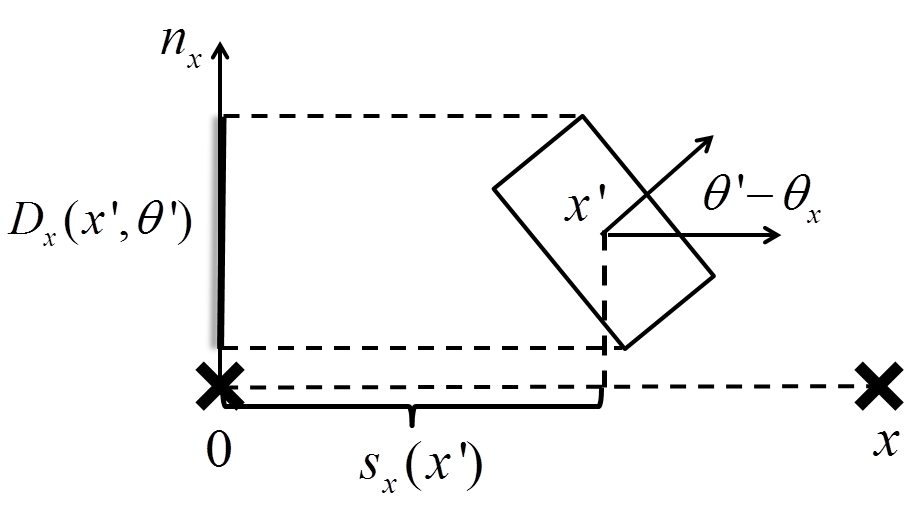
\includegraphics[width = 0.4\textwidth]{Channel_ENB.pdf}
	\caption{User $(x', \theta')$ will block the LOS channel between $0$ and $x$ if the projection of $x'$ lies on $x$ and the projection of his cross-segment covers $0$. }
	\label{fig:Channel_enb}
\end{figure}

Based on the geometric analysis, we can compute the probability that a user located at $x$ is a strong interferer of the typical user in the following theorem.  

\begin{theorem}\label{theorem:E_N_B_LOS}
	The number of users blocking $l_{0,x}^{\mathrm{LOS}}$, $N_\mathrm{B}^\mathrm{LOS}(x)$, follows Poisson distribution and the average number of blockage $\mathrm{E}[N_{\mathrm{B}}^\mathrm{LOS}(x)] \approx \lambda |x| \mathrm{E}[D]$. $\mathrm{E}[D]$ is the expected width of cross section of user.  
\end{theorem}
\begin{proof}
	The number of blockages is given by,
	\begin{equation*}
	N_{\mathrm{B}}^\mathrm{LOS}(x) = \sum_{(x_i, \theta_i)\in \tilde{\Phi}\backslash(x,\theta)}1\big((x_i, \theta_i) \mathrm{~blocks~} l_{0,x}^{\mathrm{LOS}}\big).
	\end{equation*}
	$\tilde{\Phi}\backslash(x,\theta)$ is an independently marked PPP and $1\big((x_i, \theta_i) \mathrm{~blocks~} l_{0,x}^{\mathrm{LOS}}\big)$ only depends on $(x_i, \theta_i)$. $N_{\mathrm{B}}(x)$ is an independently thinned Poisson process, which is still a Poisson process \cite{stochasticgeometry}. 
	
	\begin{align}
	\mathrm{E}[N_{\mathrm{B}}^\mathrm{LOS}(x)] & =  \int\limits_{\mathbb{R}^2}\int\limits_{[0,2\pi)}\mathrm{1}((x',\theta')\mathrm{~blocks~}(x,\theta))F_{\theta'}(\mathrm{d}\theta')\lambda(\mathrm{d}x') \nonumber\\
	& \stackrel{(a)}{\approx} \int\limits_{\mathbb{R}^2}\int\limits_{[0,2\pi)}\mathrm{1}\big(0\notin D_x(x',\theta')\big) \nonumber\\
	& \phantom{{}=1} \times \mathrm{1}\big(s_{x}(x')\in[0,|x|]\big) F_{\theta'}(\mathrm{d}\theta')\lambda(\mathrm{d}x') \label{eq:2dblocking} \\
	& \stackrel{(b)} = \lambda|x|\int\limits_{[0,2\pi)}|D_x(\cdot, \theta')| F_{\theta'}(\mathrm{d}\theta') \nonumber\\
	& \stackrel{(c)} = \lambda|x|\mathrm{E}[|D_x|] \label{eq:N_blockage_original}
	\end{align}
	where in (a), we use the two conditions of projections to approximate $\mathrm{1}((x',\theta')\mathrm{~blocks~}(x,\theta))$. In (b), we use the fact that users follows HPPP with density $\lambda$. The location the dimensions of users are independent of the locations of users thus the distribution of $|D_x(x', \theta')|$ is independent of $x'$. In (c), $\mathrm{E}[|D_x|]$ is the expectation of $B_x$ over user orientations. If the orientations of users is uniform over $[0, 2\pi)$, then $\mathrm{E}[|D_x|]$ is the same for all $x$. Denote $\mathrm{E}[D] = \mathrm{E}[|D_x|]$ and this finishes the proof.
\end{proof}

By Theorem \ref{theorem:E_N_B_LOS}, the probability that $l_{0,x}^{\mathrm{LOS}}$ is blocked over $\mathbb{\tilde{M}}$ is given by $e^{-E[N_\mathrm{B}^\mathrm{LOS}(x)]}$. For LOS channel, $f_0$ can be written as, 
\begin{multline}\label{eq:f0_LOS}
	f_0(x,\theta, \tilde{\phi},\theta_0)=\text{1}((x,\theta)\mathrm{~faces~}(0,\theta_0))\cdot\mathrm{1}(N_\mathrm{B}^\mathrm{LOS}(x)=0) \\
	\cdot\text{1}(|x|\leq r_{\max}). 
\end{multline}

Considering the fact that users can not overlap with the typical user, the users that are too close to the typical should not be included in $N_{\mathrm{SI}}$, thus we integrate over $\mathbb{R}\backslash{\mathcal{B}(0, r_{\min})}$ where $\mathcal{B}(0, r_{\min})$ is a circle centered at $0$ with a radius $r_{\min}$ and $r_{\min}$ is the minimum distance between users. 
$\mathrm{E}[N_{\mathrm{SI}}^{\text{LOS}}]$ is as follows, 
\begin{equation}
\begin{aligned}
\mathrm{E}[N_{\mathrm{SI}}^{\text{LOS}}] &= \int\limits_{\mathbb{R}^2\backslash\mathcal{B}(0,r_{\text{min}})} \int\limits_{[0,2\pi)}\mathrm{E}_{\theta_0}[\text{1}((x,\theta)\mathrm{~faces~}(0,\theta_0))]\\
& \phantom{{}=1} \cdot\text{1}(|x|\leq r_{\max})\cdot e^{-\mathrm{E}[N_{\mathrm{B}}^\mathrm{LOS}(x)]}F_{\theta}(\mathrm{d}\theta)\lambda(\mathrm{d}x)\\
& \stackrel{(a)} = \int\limits_{\mathbb{R}^2\backslash\mathrm{B}(0,r_{\text{min}})}
\mathrm{P}_{\text{facing}}(x)\text{1}(|x|<r_{\text{max}})e^{-\mathrm{E}[N_{\mathrm{B}}^\mathrm{LOS}(x)]}\lambda(\mathrm{d}x)\\
& = 2\pi\lambda \mathrm{P}_{\text{facing}}\int\limits_{\mathrm{r_{min}}}^{\mathrm{r_{max}}}e^{-\lambda\cdot\mathrm{E}[D]\cdot r}r\mathrm{d}r\\
& =\frac{2\pi \mathrm{P}_{\text{facing}}}{\lambda \mathrm{E}[D]^2}\big( e^{-\lambda\mathrm{E}[D]r_{\mathrm{min}}}(\lambda\mathrm{E}[D]r_{\mathrm{min}} + 1)\\
& \phantom{{}=1} - e^{-\lambda\mathrm{E}[D]r_{\mathrm{max}}}(\lambda\mathrm{E}[D]r_{\mathrm{max}} + 1)\big)
\end{aligned} 
\end{equation}
In (a), $\mathrm{P}_{\text{facing}}$ is the probability that the link is not blocked by the typical user or the user $(x,\theta)$, i.e.,
\begin{equation*}
\mathrm{P}_{\text{facing}}(x) = \int\limits_{[0,2\pi)}\mathrm{E}_{\theta_0}[\text{1}((x,\theta)\mathrm{~faces~}(0,\theta_0))]F_{\theta}(\mathrm{d}\theta)
\end{equation*}
$\theta_0$ and $\theta$ are uniform over $[0, 2\pi)$, thus $\mathrm{P}_{\text{facing}}(x)$ is same for all $x$.

For NLOS channel, the number of blockages also follows Poisson distribution. We can compute $\mathrm{E}[N_{\mathrm{B}}^{\mathrm{NLOS}}]$ in a similar way as above for  $\mathrm{E}[N_{\mathrm{B}}^\mathrm{LOS}(x)]$ by substituting the first indicator function in (\ref{eq:2dblocking}), $\mathrm{1}\big(0\notin B_x(x',\theta')\big)$, with 
$$\mathrm{1}\big(h_{x}(x',\theta_{x'}) > h_{\mathrm{NLOS}}(x, s_x(x'))  \big),$$
where $h_{x}(x',\theta_{x'}) $ is the height of user of $x'$ along $x$. $h_{\mathrm{NLOS}}(x, s_x(x'))$ is the height of the reflection channel as shown in Fig. \ref{fig:NLOS}. 
\begin{figure}
	\centering
	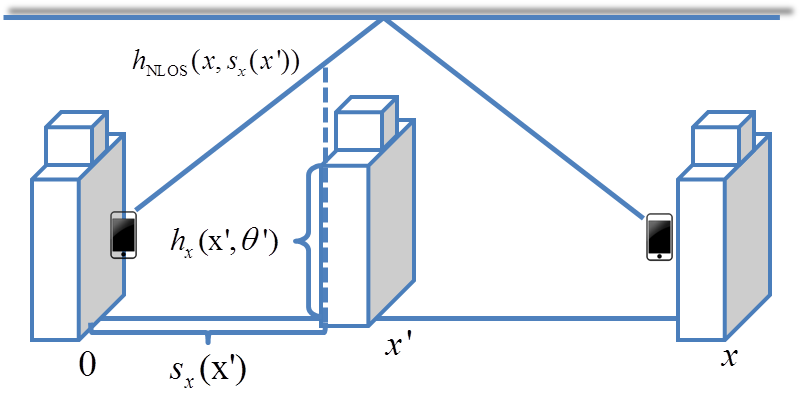
\includegraphics[width = 0.4\textwidth]{Channel_NLOS.pdf}
	\caption{User $x$ has a clear reflected channel if there is no other user blocking the reflection path, i.e., there is no user $(x',\theta')$ such that $\{s_x(x')\in [0, |x|]\}\cap\{ h_x(x', \theta') \geq h_{\mathrm{NLOS}}(x, s_x(x'))\}$.}
	\label{fig:NLOS}
\end{figure}

We make further assumptions about users that user bodies are cylinders, or more generally, the cross section of user body at height $h_1$, $\sigma(h_1)$, is contained in the cross section of user body at height $h_2$, $\sigma(h_2)$, for $h_1\geq h_2\geq h_{\mathrm{device}}$, i.e., 
\begin{equation}\label{condition1}
\sigma(h_1)\subseteq \sigma(h_2), \forall h_1\geq h_2\geq h_{\mathrm{device}}.
\end{equation}

If the users satisfies the condition in (\ref{condition1}), then a user that does not block $l_{0,x}^{\mathrm{LOS}}$ does not block $l_{0,x}^{\mathrm{NLOS}}$, i.e., $x\cap \sigma(h_{\mathrm{device}}) = \emptyset$, then $x\cap \sigma(h') = \emptyset$ for $h'>h_{\mathrm{device}}$.

Combining the above results, the expected number of strong interferers is given by 
\begin{multline}\label{eq:E_N_SI}
	\mathrm{E}[N_{\mathrm{SI}}] =  \int\limits_{\mathbb{R}^2}
	\mathrm{P}_{\text{facing}}(x)\\
	\cdot \big[\text{1}(|x|\in[r_{\min},r_{\text{max}}^{\mathrm{reflection}}])
	\cdot e^{-\mathrm{E}[N_{\mathrm{B}}^\mathrm{NLOS}(x)]} \\
	 + \text{1}(|x|\in[r_{\text{max}}^{\mathrm{reflection}},r_{\text{max}}])
	 \cdot e^{-\mathrm{E}[N_{\mathrm{B}}^\mathrm{LOS}(x)]} \big]\lambda(\mathrm{d}x)
\end{multline}


\subsection{Sensitivity of Strong Interferers}\label{section:channel:sensitivity}
In this section we introduce local movements model and study the sensitivity of strong interferers to users' small local movements.
The sensitivity of strong interferers, i.e., how strong interferers changes when users move, defines the cost and benefit of keep tracking of and coordinating the strong interferers and how robust the strong interferers are to perturbations in the network. Suppose in a time interval $[t, t+ \Delta t]$, users make translations as well as rotations, resulting in changes for the typical user and potential interferers summarized as follows:
\begin{equation*}
\begin{split}
(0,\theta_0)&\rightarrow(\Delta x_0, \theta_0 + \Delta\theta_0) \\
\tilde{\Phi}^{t}=\{(x_i, \theta_i)\}&\rightarrow\tilde{\Phi}^{t+\Delta t}=\{(x_i+\Delta x_i, \theta_i + \Delta\theta_i)\}
\end{split}
\end{equation*}

Let $Y_x^t=f_0(x, \theta, \tilde{\Phi}^t\backslash (x, \theta), \theta_0)$ be the state of the interferer located at $x$ at time $t$, and $Y_x^{t+\Delta t}$ be the state of the same user at $t+\Delta t$, which is given by,
\begin{multline*}
Y_{x}^{t+\Delta t} = f_{\Delta x_0}(x+\Delta x, \theta + \Delta\theta, \tilde{\Phi}^{t+\Delta t}\backslash (x+\Delta x, \theta + \Delta\theta), \\
\theta_0 + \Delta\theta_0),
\end{multline*}
$Y_x^t \mathrm{~and~} Y_{x}^{t+\Delta t} \in \{0,1\}$. $Y = 1$ if the user is a strong interferer of the typical user and $Y = 0$ otherwise. We define the sensitivity of an interferer originally located at $x$ for an interval of length $\Delta t$, $S(x, \Delta t)$, via the autocorrelation of the state of the interferer at $t$ and $t+\Delta t$, 
\begin{equation}
S(x, \Delta t)
=\mathrm{Corr}(Y_x^t, Y_x^{t+\Delta t})
=\frac{\mathrm{E}[Y_x^t\cdot Y_x^{t + \Delta t}]}{\sigma_{Y_x^t}\cdot \sigma_{Y_x^{t+\Delta t}}},
\end{equation}
$S(x, \Delta t)\in [0,1]$. If $S(x, \Delta t)$ is small, the autocorrelation between the state of the channel is small and sensitive to movements; if $S(x, \Delta t)$ approximates $1$, the autocorrelation is high and the strong interferer is stable.

%We assume the locations of users follow HPPP of density $\lambda$ and the users make movements independent of their locations. For the orientations of users, we assume $\tilde{\Phi}$ is i.m.p.p. and $\theta \sim \unif(0,2\pi)$, also the rotation of users is independent of users' orientations. 

%To compute $S(x, \Delta t)$, we need to know the distribution of users in presence of movements. We assume users are uniformly distributed on the plane and users make independent movements, then we have the following theorem on the $\Phi$.

Based on our assumptions on $\tilde{\Phi}$ and independent movements, we have the following theorems on the state of the network after user moves.

\begin{theorem}\label{theorem:hppp}
If $\Phi^t$ is HPPP with density $\lambda$ and users make independent movements and the movements is indepedent of users' location, then $\Phi^{t+\Delta t}$ is still HPPP with density $\lambda$. 
\end{theorem} 
\begin{proof}
Let $p_{t, t+\Delta t}(x, x+\Delta x)$ be the probability that the user located at $x$ at time $t$ moves to $x + \Delta x$ at time $t+\Delta t$. Users' movements are independent and the movements are independent of $x$, then $p_{t, t+\Delta t}(x, y)$ is a function of $\Delta x$, i.e., $p_{t, t+\Delta t}(x, x+\Delta x) = g_{t, t+\Delta t}(\Delta x)$.
According to the displacement theorem in \cite{poisson}, $\Phi^{t+\Delta t}$ is a HPPP with density $\lambda$.
\end{proof}

\begin{theorem}\label{theorem:hppp_orientation}
$\tilde{\Phi}^{t+\Delta t}$ is an i.m.p.p. and $\theta$ is uniform in $[0, 2\pi)$ at $t+ \Delta t$. 
\end{theorem}
\begin{proof}
	$\theta$ and $\Delta \theta$ are independent from other users and the locations and translations of users, $x$ and $\Delta x$, thus $\tilde{\Phi}^{t+\Delta t}$ is i.m.p.p.. If $\theta^t\sim \unif(0, 2\pi)$ and $\Delta \theta$ is independent from $\theta^t$, then follow the similar proof used in displacement theorem, $\theta^{t + \Delta t}\sim \unif(0, 2\pi)$. 
\end{proof}

By Theorem \ref{theorem:hppp} and \ref{theorem:hppp_orientation}, $\tilde{\Phi}$ is stationary and the variance of $Y_x^t$ and $Y_x^{t+\Delta t}$ are the same and independent of $t$ or $\Delta t$ if we ignore the change in $|x|$,  
\begin{equation*}
\mathrm{Var}(Y_x)=p_{\mathrm{SI}}(x)\cdot (1-p_{\mathrm{SI}}(x)),
\end{equation*}
where $p_{\mathrm{SI}}(x)=\mathrm{Pr}(f_0(x,\theta,\tilde{\Phi}\backslash\{(x_i,\theta_i)\}, \theta_0)=1)$. 

By definition, 
\begin{equation*}
\mathrm{E}[Y_x^t\cdot Y_x^{t + \Delta t}] = \mathrm{Pr}(\{Y_x^t=1\}\cap \{Y_x^{t+\Delta t}=1\}),
\end{equation*}
is the probability that user at $x$ is strong interferer at $t$ and $t + \Delta t$. The movements of users during $\Delta t$, $(\Delta x, \Delta \theta)$ can be counted as marks of $\Phi$, and the new m.p.p. is $\tilde{\Phi}^{\Delta t} = \{(x_i, m_i)\}_i$, where $m_i = (\theta_i, \Delta x_i, \Delta \theta_i)$ is the new marks of the point process. According to our assumptions of independently marked process, $\tilde{\Phi}^{\Delta t}$ is an i.m.p.p.. 

Denote $f_0^{\Delta  t}(x_i, m_i, \tilde{\Phi}^{\Delta t}\backslash (x_i, m_i), m_0)$ be the indicator function that the user located at $x$ is a strong interferer at $t$ and $t + \Delta t$, then 
\begin{multline*}
f_0^{\Delta  t}(x_i, m_i, \tilde{\Phi}^{\Delta t}\backslash (x_i, m_i), m_0) = \\
f_0(x,\theta, \tilde{\Phi}, \theta_0) 
\cdot f_{\Delta x_0}(x+\Delta x,\theta + \Delta \theta, 
\\ \tilde{\Phi} + \Delta \tilde{\Phi}\backslash (x+\Delta x,\theta + \Delta \theta), \theta_0+\theta_0),
\end{multline*}
where $\Delta \tilde{\Phi} = \{(\Delta x_i, \Delta \theta_i)\}_i$ is the movement of users during $\Delta t$ and we denote $\tilde{\Phi} + \Delta \tilde{\Phi} = \{(x_i+\Delta x_i, \theta_i + \Delta \theta_i)\}_i$ as the network after users move.  
Given the model of movements, i.e., $F_{(\Delta x, \Delta \theta)}$, we can compute $\mathrm{E}[f_0^{\Delta t}]$ using the same technique used in the previous section. 


\subsection{Influence of Mobile Blockers on Static Wearable Networks}\label{subsection:largemobility}
Another scenario we are interested in is the dense user environment where some users move and the other users stay fixed, e.g., in a train cart, some users are sitting in their seats while other users are leaving the train through the passage. 
In this section we study the influence of mobile blockers on static channels. We assume the blockages make constant velocity movements towards their orientation and we refer to the model as Constant Velocity Model(CVM).

For CVM, we focus on whether the channel is LOS channel, thus we place the users on the 2-D plane. 
We first introduce the following operations on subsets $A, B\in \mathbb{R}^2$ in \cite{stochasticgeometry}, 
\begin{equation*}
\begin{split}
A \oplus B & = \{x+y:x\in A, y\in B\},\\
x + B & = \{x+y:y\in B\}, \mathrm{~for~} x\in \mathbb{R}^2, \\
\check{B} & = \{x: -x \in B\}.
\end{split}
\end{equation*}

Now we describe the assumptions about CVM in detail. At time $0$, the locations of users, $\Phi^0 = \{x_i^0\}_i$, follows HPPP with density $\lambda$, and the orientations of users is independently and uniformly distributed in $[0, 2\pi]$, $\theta_i \sim \unif(0, 2\pi)$. Users moves towards their orientation at constant velocities $\{s_i\}_i$ and $s_i$'s are independently and identically distributed (i.i.d.).

Assume $A_0^{\theta_i}$ is convex and bilateral symmetrical \underline{along} $\theta_i$ and the width of $A_0$ is $D_0$. $x_i^t$ is the location of the center of $u_i$ at time $t$, then the area $u_i$ blocks at time $t$, $\Xi_{i}^t$, is given by 
\begin{equation*}
\Xi_{i}^t = x_i^t + A_0^{\theta_i}.
\end{equation*}
From $t$ to $t+\Delta t$, $u_i$ moves from $x_i^t$ to $x_i^{t+\Delta t} = x_i^t + \vec{s}_i\cdot \Delta t$ and we denote the $l_{x_i^t, x_i ^{t+\Delta t}}$ as the trace of the center of $u_i$. The area that $u_i$ covers during $[t, t+\Delta t]$, $\Xi_i^{[t, t+\Delta t]}$, is as follows, 
\begin{equation*} %\label{eq:cover_area}
\Xi_i^{[t, t+\Delta t]} = A_0^{\theta_i} \oplus l_{x_i^t, x_i ^{t+\Delta t} }.
\end{equation*}
Fig. \ref{fig:boolean} illustrates the boolean model of mobile blockages.

\begin{figure}
	\centering
	\mbox{\subfloat[]{\label{subfig:trace} 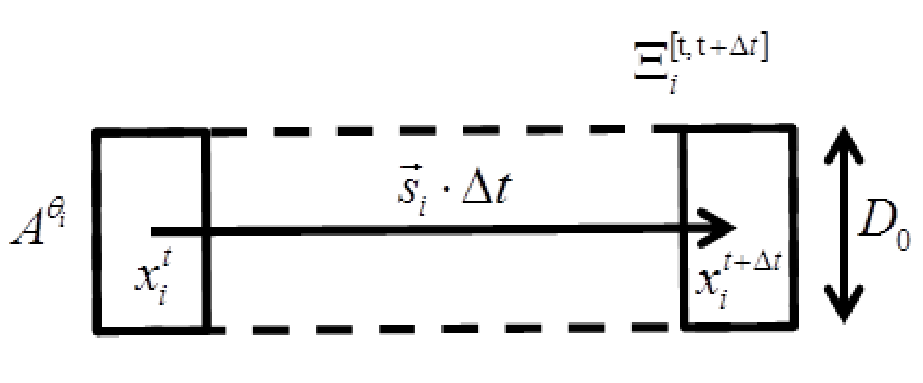
\includegraphics[width=0.3\textwidth]{Channel_trace.pdf}}}
	\mbox{\subfloat[]{\label{subfig:boolean} 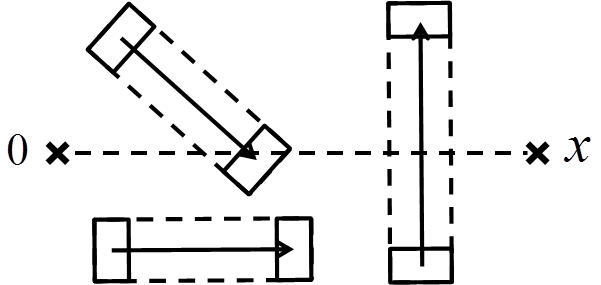
\includegraphics[width=0.3\textwidth]{Channel_boolean.pdf}}}
	\caption[]{\subref{subfig:trace} shows the $\Xi_i^{[t, t+\Delta t]}$. If $A_0^{\theta_i}$ is convex then $\Xi$ is also convex. In \subref{subfig:boolean} $u_i$ blocks channel in $[t, t+ \Delta t]$ if $\Xi_i^{[t, \Delta t]}\cap x \neq \emptyset$. }
	\label{fig:boolean}
\end{figure}

The distribution of user locations and velocities is given in the following theorem.
\begin{theorem}\label{theorem:boolean_stationary}
Suppose users make i.i.d. constant velocity movements and the locations of users follows HPPP at time $0$, then $\tilde{\Phi}_c^t = \{(x_i^t, (\theta_i, s_i))\}_i$ is stationary.
\end{theorem}
The proof uses displacement theory and is similar to the proof of Theorem \ref{theorem:hppp} and \ref{theorem:hppp_orientation}.
By Theorem \ref{theorem:boolean_stationary}, 

$\Xi_i^{[t, t+\Delta t]}$ is i.i.d. distributed and independent of $x_i^t$ thus we can use the Boolean Model \cite{stochasticgeometry} to model the area that users have covered during $[t, t+\Delta t]$, i.e., 
\begin{equation*}
\tilde{\Phi}_{\Xi}^{[t, t+\Delta t]} = \{(x_i^t, \Xi_i^{[t, t+\Delta t]})\}_i.
\end{equation*}
The set of users that has blocked channel $x$ during $[t, t+\Delta t]$ is given by
\begin{equation*}
N_{\mathrm{B}}^{[t, t + \Delta t]} = \{x_i:x_i \in \Phi, \Xi_i^{[t, t+\Delta t]}\cap x \neq \emptyset \}.
\end{equation*}
For the boolean model, $|N_{\mathrm{B}}^{[t, t + \Delta t]}|$ is a Poisson random variable with parameter $\lambda\mathrm{E}[\nu_2(\check{x}\oplus \Xi_i^{[t, t+\Delta t]})]$, where $\nu_2$ is the area of the set \cite{stochasticgeometry}.

$A_0^{\theta_i}$ is bilateral symmetric, $\theta_i\sim\unif(0, 2\pi)$ and $s_i$ is independent from $\theta_i$, thus $\tilde{\Phi}_{\Xi}^{[t, t+\Delta t]}$ is isotropic. For isotropic $\Xi_i^{[t, t+\Delta t]}$ and $\Phi^t$ following HPPP with density $\lambda$, we have the following theorem for $\mathrm{E}[\nu_2(\check{x}\oplus\Xi_i^{[t, t+\Delta t]})]$.

\begin{theorem}\label{theorem:boolean_mean}
$K$ is a closed convex set and $\Xi_0$ is convex and isotropic. In two dimensional case, the average number of germs intersects  with $K$ is $\lambda\mathrm{E}[\nu_2(\check{K}\oplus \Xi_0)]$, where 
\begin{equation}\label{eq:interference:boolean_mean}
\mathrm{E}[\nu_2(\check{K}\oplus \Xi_0)] = \nu_2(K) + \mathrm{E}[\nu_2(\Xi_0)] + \frac{1}{2\pi}\nu_1(K)\mathrm{E}[\nu_1(\partial \Xi_0)],
\end{equation}
$\nu_1$ is the one-dimensional measure and $\partial \Xi_0$ is the boundary of $\Xi_0$.
\end{theorem}
Theorem \ref{theorem:boolean_mean} is the two-dimensional capacity functional given by (3.31) in \cite{stochasticapp}, where (\ref{eq:interference:boolean_mean}) is the planar case of the generalized Seiner formula (6.29) in \cite{stochasticapp},  
\begin{equation*}
\E\big[\nu_d(\Xi\oplus K)\big] = \frac{1}{b_d}\sum\limits_{k=0}^{d}\frac{b_k b_{d-k}}{{d \choose k}}\overbar{V}_k(\Xi) V_{d-k}(K),
\end{equation*}
% b_d is the measure of unit ball in R^d
$d$ is the dimension, $b_k$ is the measure of unit ball in dimension $k$, $V_k$ is the intrinsic volume in dimension $k$ and $\overbar{V}_k(\Xi) = \E[V_k(\Xi)]$ is mean intrinsic volume of $\Xi$ in dimension $k$. We present the proof in appendix.

By Theorem \ref{theorem:boolean_mean} and making $K = x$, we can compute $\E[\nu_2(\check{x}\oplus\Xi_0^{[t, t+\Delta t]})]$ as follows,
\begin{equation}\label{eq:boolean_mean}
\E[\nu_2(\check{x}\oplus\Xi_0^{[t, t+\Delta t]})] = \E[\nu_2(\Xi_0^{[t, t+\Delta t]})] + \frac{|x|}{\pi}\E[\nu_1(\partial \Xi_0^{[t + \Delta t}])],
\end{equation}
where
\begin{equation*}
\begin{split}
\E[\nu_2(\Xi_0^{[t, t+\Delta t]})] & = \nu_2(A_0) + D_0\E[s]\Delta t,\\
\E[\nu_1(\Xi_0^{[t, t+\Delta t]})] & = \nu_1(A_0) + 2\E[s]\Delta t.
\end{split}
\end{equation*}

Now we can compute the probability that channel $x$ is not blocked as follows, 
\begin{equation}\label{eq:P_LOS}
\begin{aligned}
\mathrm{P}_{\mathrm{LOS}} & = \mathrm{P}(N_{\mathrm{B}}^{[t, t]}=0)  \\
& = e^{-\E[N_\mathrm{B}^{[t,t]}]} \\
& = e^{-\lambda(\nu_2(A_0) + \frac{|x|}{\pi}\nu_1(A_0))}. 
\end{aligned}
\end{equation}

Armed with the analysis for the number of users that have blocked channel during any time interval, we now analyze the dynamics of the state of channel. We model channel $x$ as a queue, $Q$, while the blockages are modeled as the jobs coming to the queue. 
The service time $S$ is the time that a blockage blocks the channel. $S$ is related to $x_i$, $\theta_i$ and $s_i$ thus the service time can be viewed as following a general distribution. Since we assume that the movements of users are independent from each other, the time that each blockage blocks the channel (stays in the queue) is independent from others thus $Q$ has infinite servers. For the number of new blockages (NB) that begin to block channel $x$ during $[t, t+\Delta t]$, $N_{\mathrm{NB}}^{[t, t+\Delta t]}$, we have the following theorem.

\begin{theorem}\label{theorem:poisson_arrival}
For CVM, $N_{\mathrm{NB}}^{[t, t+\Delta t]}$ follows a Poisson distribution with density $\lambda\E[s](D_0 + 2|x|/\pi)\Delta t.$
\end{theorem}
\begin{proof}
The users that begins to block channel $x$ during $[t, t+\Delta t]$ is an independent thinning of a PPP, thus $N_{\mathrm{NB}}^{[t, t+\Delta t]}$ follows a Poisson distribution. 

The number of users that begins to block the channel is the number of users that has blocked channel $x$ during $[t, t+\Delta t]$ minus the number of blockages at $t$,  
\begin{equation*}
\begin{aligned}
N_{\mathrm{NB}}^{[t, t+\Delta t]} & = N_\mathrm{B}^{[t, t+\Delta t]} - N_\mathrm{B}^{[t, t]} \\
\E[N_{\mathrm{NB}}^{[t, t+\Delta t]}] & = \E[N_\mathrm{B}^{[t, t+\Delta t]}] - \E[N_\mathrm{B}^{[t, t]}] \\
									  & = \lambda\E[s](D_0 + 2|x|/\pi)\Delta t.
\end{aligned}
\end{equation*}
\end{proof}

By Theorem \ref{theorem:poisson_arrival}, the arrival of blockages is memoryless.  Given the above analysis, $Q$ is a $M/GI/\infty$ queue,  and the arrival rate of blockages, $\lambda^Q$ is as follows,
\begin{equation}\label{eq:lambda_queue}
\lambda^Q = \lambda\E[s](D_0 + 2|x|/\pi).
\end{equation} 

Let $T_{\mathrm{LOS}}$ be a random variable denoting the time a LOS link is available in steady state and $T_{\mathrm{NLOS}}$ be the time that the channel stays blocked. For $M/G/\infty$ queue, $T_{\mathrm{LOS}}$ follows a exponential distribution with parameter $\lambda^Q$, thus $\E[T_{\mathrm{LOS}}]$ is given by, 
\begin{equation}\label{eq:T_LOS}
\E[T_{\mathrm{LOS}}] = \frac{1}{\lambda\E[s](D_0 + \frac{2|x|}{\pi})}.
\end{equation}
The distribution of $Q$'s busy period $T_{\NLOS}$ is difficult to derive and related to $A_0$ and the distribution of $s$, thus we focus on $\E[T_{\mathrm{NLOS}}]$ to see how user mobility influence the blocked period of the channel. The system is stationary thus we have the following relationship between $\mathrm{P}_{\LOS}$, $\E[T_{\LOS}]$ and $\E[T_{\NLOS}]$, 
\begin{equation}\label{eq:t_relation}
\mathrm{P}_{\LOS} = \frac{\E[T_{\LOS}]}{\E[T_{\LOS}] + \E[T_{\NLOS}]}.
\end{equation}
From (\ref{eq:t_relation}), we can derive $\E[T_{\NLOS}]$ as follows, 
\begin{equation*}\label{eq:T_NLOS}
\E[T_{\NLOS}] = \frac{1-\mathrm{P}_{\LOS}}{\mathrm{P}_{\LOS}}\E[T_{\LOS}],
\end{equation*}
where $\mathrm{P}_{\LOS}$ is given in (\ref{eq:P_LOS}) and $\E[T_{\LOS}]$ is given in (\ref{eq:T_LOS}).

Based on the results of $\E[T_{\LOS}]$ and $\E[T_{\NLOS}]$, we can compute the frequency that the state of channel changes from LOS to NLOS then back to LOS, $f_{\mathrm{change}}$, as follows,
\begin{equation*}\label{eq:frequency}
f_{\mathrm{change}} = \frac{1}{\E[T_{\LOS}] + \E[T_{\NLOS}]}.
\end{equation*}  

In some cases we can get more information about the distribution of $T_{\NLOS}$. If the time that each user blocks the channel is equal, e.g., all users have the same orientation and velocity, $Q$ becomes an $M/D/\infty$ queue and the distribution of busy period is given in \cite{busyperiod_heavytraffic}. The author of \cite{busyperiod_heavytraffic} also shows that the busy period of $M/GI/\infty$ queue is asymptotically exponential with mean equal to expected busy period if the distribution function of service time, $H$, satisfies that,  
\begin{equation}\label{eq:busyperiod_condition}
(\log z) \int_{z}^{\infty}\{1-H(y)\}\mathrm{d}y\rightarrow 0,
\end{equation}
as $z\rightarrow \infty$. 
For our constant velocity model, we derive a sufficient condition for busy period to approximate exponential distribution in the following theorem.

\begin{theorem}\label{theorem:T_NLOS_exp}
For CVM, the distribution of $T_{\NLOS}$ approximates exponential distribution with mean $\E[T_{\NLOS}]$ as $\lambda^Q\rightarrow \infty$ if the velocity of blockages meets following condition,
\begin{equation}\label{condition:T_NLOS_exp}
s_i\geq s_{\min}, s_{\min}>0,
\end{equation} 
for all blockage $i$.
\end{theorem}

\begin{proof}
$s_i>s_{\min}$ then service time $S_i$ is bounded by $(|x|+d_A)/s_{\min}$, where $d_A$ is the diameter of the smallest circle that cover contains $A$. $H(y) = 1$ for $y>(|x|+d_A)/s_{\min}$ thus (\ref{eq:busyperiod_condition}) is satisfied. By Theorem 1 in \cite{busyperiod_heavytraffic}, 
\begin{equation*}
\mathrm{P}(\E[T_{\NLOS} \leq z\E[N_{\NLOS}]]) \rightarrow 1-e^{-z}, z>0,
\end{equation*} 
as $\lambda^Q\rightarrow \infty$.
\end{proof}

Theorem \ref{theorem:T_NLOS_exp} indicates that the exponential distribution is a good approximation for $T_{\NLOS}$ if $\lambda^Q$ is large. From (\ref{eq:lambda_queue}), we know that $\lambda^Q$ is large if user density is high, user speed is large and channel $x$ is long. \cite{busyperiod_exponential} provides some other conditions when the distribution of busy period is approximately exponentially distributed.
 
If $\lambda^Q$ is small, exponential distribution may not fit $T_{\NLOS}$ well. For example, if $\lambda^Q$ is very small, the probability that the channel is blocked by more than one blockage is small and the distribution of $T_{\NLOS}$ can be approximated by the distribution of $S$.

% low arrival rate case; movement of transceivers, 
Coupling of blockages?


\section{Numberical Results for Interference Environment and Implications on MAC design} \label{section:channel_numerical}
In this section, we show the numerical results for our analysis in Section \ref{section:channel} and discuss the implications of the interference environment on MAC design. 

We first compute $\mathrm{E}[N_{\mathrm{SI}}]$ for simple user body model, in which we model users as cylinders with a diameter of 0.6 m. We then compare the analytical results with simulations. In dense environment, the volume of human body is not negligible and the distribution of users will be more organized as user density increases since there will be some minimum distance between users. To evaluate how much this factor affects our the accuracy of our analysis, we use Mat\'ern \Rom{3} process \cite{matern} to model the locations of users and instead of HPPP. The height of users is 1.754 m, and the height of the ceiling is $2.8$ m. The material of the ceiling is one layer polyester board with a thickness of 9 mm. We assume the users do not have a specific polarization. $r_{\max} = 10\mathrm{~m}$, at which distance the path loss of LOS channel is -88 dB, and $r_{\max}^{\mathrm{reflection}} = 3$ m. 

In Fig. \ref{fig:Channel_en_si} we show $\mathrm{E}[N_{\mathrm{SI}}]$ for different user densities. The average number of LOS and NLOS interferers are exhibited and compared to the results from simulations. In the simulation, we place the device on the surface of user body and adjust (\ref{eq:E_N_SI}) accordingly. Our analytical results are in line with the simulations, validating the accuracy of the approximation. 

\begin{figure}
	\centering
	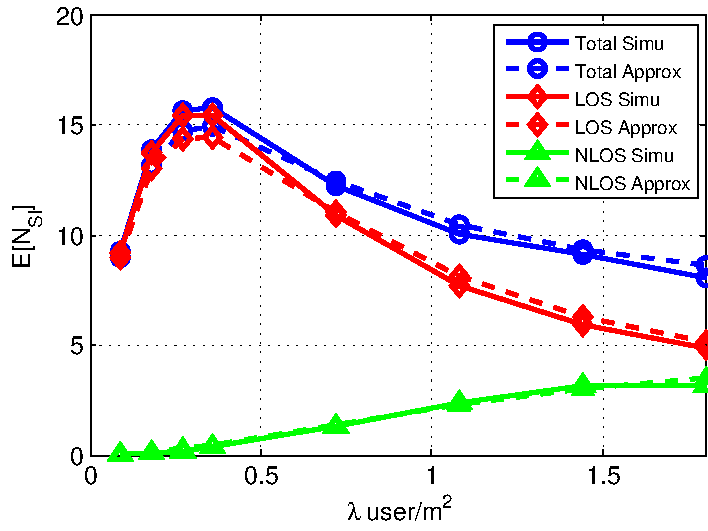
\includegraphics[width = 0.4\textwidth]{Channel_en_si.pdf}
	\caption{$\mathrm{E}[N_{\mathrm{SI}}]$ for different user densities. Whether user at $x'$ blocks the channel is decided by $h_x(x',\theta')$ and $h_{\mathrm{NLOS}}$.}
	\label{fig:Channel_en_si}
\end{figure}


\begin{figure}
	\centering
	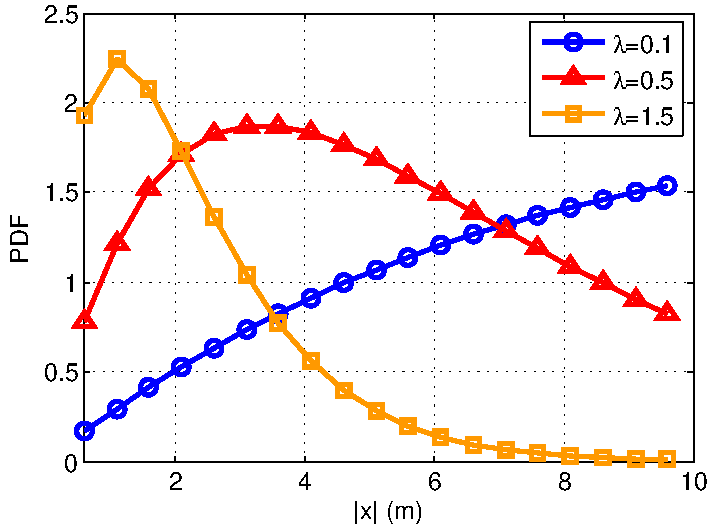
\includegraphics[width = 0.4\textwidth]{Channel_si_pdf.pdf}
	\caption{Probability density function of LOS strong interferers as a function of the distance to the typical user at $\bf{0}$.}
	\label{fig:Channel_si_pdf}
\end{figure}

As can be seen, $\mathrm{E}[N_{\mathrm{SI}}]$ first grows in the user density, but as user density further increases, users closely around the typical user form a ring blocking the interference from most users outside the ring. Also note that users see the most strong interferers at moderately high user densities. 

Fig. \ref{fig:Channel_si_pdf} illustrates how the distribution for the distance of strong interferers for varying user densities, with self blockage not considered. In high density scenario, the number of users the MAC needs to coordinate is actually limited, indicating that it is possible to mitigate interference in highly dense scenario using local coordination among users.

Next we compute the sensitivity of users at different distance when users only make local movements. We only consider LOS strong interferers in our evaluation. The movements of users during $\Delta t$ is as follows, $\Delta x$ is uniformly distributed in a disc centered at the origin with the radius of $r(\Delta t)$, $\Delta x \sim \mathrm{unif}(\mathcal{B}(0, r(\Delta t)))$, and $\Delta \theta$ is uniformly distributed in an interval, i.e., $\theta \sim \mathrm{unif}[-\omega(\Delta t), \omega(\Delta t)]$. The range of translations of users is related to user density, when $\lambda$ is small, $\Delta x$ is independent of $\lambda$; if $\lambda$ is high, $\Delta x$ decreases as $\lambda$ increases. In our simulation, $\Delta t = 1$s. How $r$ changes with $\lambda$ is plotted in Fig. \ref{fig:Channel_translation_range} and $\Delta \omega = 24\degree$.

\begin{figure}
	\centering
	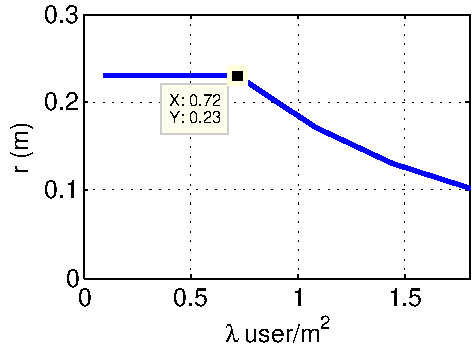
\includegraphics[width = 0.3\textwidth]{Channel_translation_range.pdf}
	\caption{Range of translation $r$ for different user densities $\lambda$. For low user density, $\lambda<0.72$, $r$ is fixed. For large $\lambda$, $r = 0.6 \sqrt{1/\lambda\pi}$ for $\lambda >0.72$.}
	\label{fig:Channel_translation_range}
\end{figure}

In Fig. \ref{fig:Channel_sensitivity}, we exhibit the sensitivity of users at different locations. Distant interferers are more sensitive to perturbations than close by interferers. This supports the observation that clusters \underline{compromising} closeby nodes (interferers) will be robust to perturbations and learning the interference form close by neighbors is more reliable. 

\begin{figure}
	\centering
	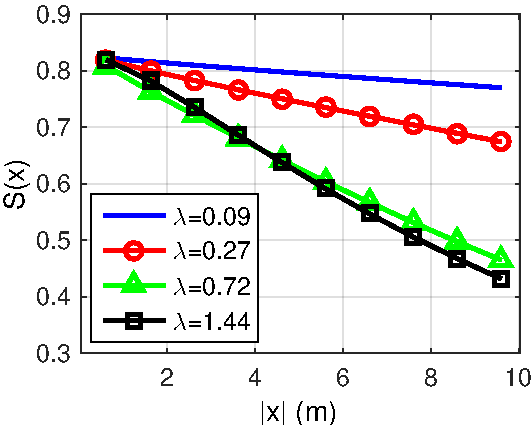
\includegraphics[width = 0.4\textwidth]{Channel_sensitivity.pdf}
	\caption{Sensitivity of users at different distances $|x|$.}
	\label{fig:Channel_sensitivity}
\end{figure}

Fig. \ref{fig:Channel_sensitivity_average} exhibits how the average sensitivity of strong interferers changes for different user densities. When user density increases, strong interferers are closer while the sensitivity of users decreases, thus the average sensitivity first decrease in the As the density of users continues to increase, this limits their range of translation and the sensitivity of users remains the same while $\mathrm{E}[S]$ increases as strong interferers are more likely to be close to the typical user. 

\begin{figure}
	\centering
	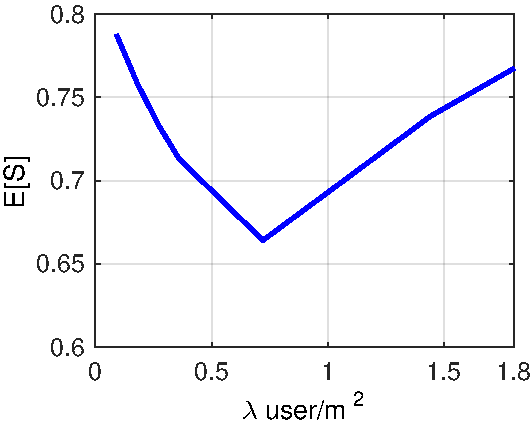
\includegraphics[width = 0.3\textwidth]{Channel_sensitivity_average.pdf}
	\caption{$\mathrm{E}[S(x)|f_0(x_i, \theta_i, \tilde{\Phi}\backslash\{(x_i,\theta_i)\}, \theta_0)=1]$ average sensitivity of strong interferers.}
	\label{fig:Channel_sensitivity_average}
\end{figure}

The above results show that interferers are more sensitive to perturbation, and thus harder to keep track of as user density increases and the worst case happens in the moderately high user density scenario, where the number of strong interferers is high and the range of perturbation is not limited by the density of users. 

\begin{figure}[htp]
	\centering
	\subfloat[$\E\lbrack T_{\LOS}\rbrack$ and $\E\lbrack T_{\NLOS}\rbrack$]{\label{subfig:et} 									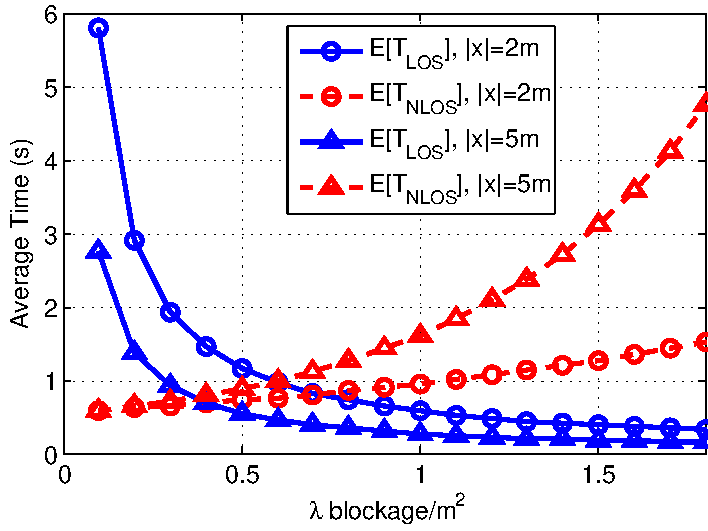
\includegraphics[width=0.4\textwidth]{Channel_constant_velocity_model.pdf} }
	
	\subfloat[State change frequency $f_{\mathrm{change}}$]{\label{subfig:freq} 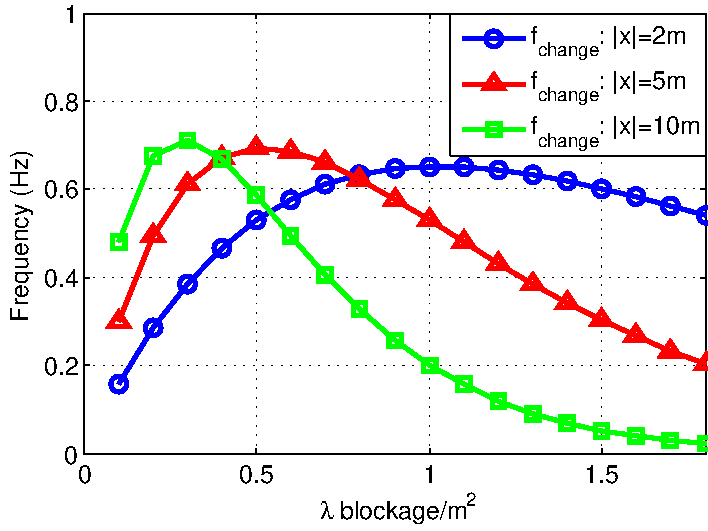
\includegraphics[width=0.4\textwidth]{Channel_constant_velocity_model_frequency.pdf}}
	
	\caption[]{$\E[T_{\LOS}]$, $\E[T_{\NLOS}]$ and $f_{\mathrm{change}}$ for different $\lambda$ and $|x|$. User's average velocity is $\E[s] = 1$m/s. Blockage is modeled as a rectangle of size $0.45\mathrm{m}\times 0.25\mathrm{m}$ and the width towards moving direction is $D_0=0.45\mathrm{m}$. }
	\label{fig:Channel_constant_velocity_model}
\end{figure}
In Fig. \ref{fig:Channel_constant_velocity_model} we present how $\E[T_{\LOS}]$, $\E[T_{\NLOS}]$ and $f_{\mathrm{change}}$ changes for different blockage density $\lambda$ and channel lengths $|x|$. From (\ref{eq:T_LOS}) we know that $\E[T_{\LOS}]$ is inversely proportional to $\lambda\E[s]|x|$ if we ignore $D_0$. Results in Fig. \ref{fig:Channel_constant_velocity_model}\subref{subfig:et} indicate that if the blockage density is higher, the blockages move faster and the link is longer, then the time of having LOS channel decreases while the time of having NLOS channel increases. Results in Fig. \ref{fig:Channel_constant_velocity_model}\subref{subfig:freq} indicate that the state of channel changes most frequently at moderately high user densities. In dense wearable networks, distant users are likely to be blocked and state of their channel is relatively stable thus we may ignore theses users in MAC protocol.

\section{MAC in Dense Wearable Networks}\label{section:MAC}
In this section, we discuss the MAC design for dense wearable networks. Devices on each user forms a PBSS and it is possible that there is no centralized access point to coordinate the massive PBSSs. In such a case, clustering is as a viable solution to organizing the PBSSs.

The 802.11ad standard provides a hierarchical MAC geared at coordinating the personal basic service sets (PBSSs). The devices of a user forms a PBSS with a device working as the PBSS coordinate point (PCP). PCPs may use the PCP clustering mechanism to improve the spatial sharing and interference mitigation with other co-channel directional multi-gigabit (DMG) BSSs. Multiple PBSSs form a cluster, with one PCP selected as the synchronization PCP (S-PCP), which can be viewed as the cluster head.
%There are two types of clustering, decentralized PCP/AP clustering and centralized PCP/AP clustering. Centralized clustering requires synchronization and coordination of multiple S-APs, which might be hard to achieve in wearable networks with unstable channels thus we focus on the decentralized clustering. 

In the decentralized clustering of 802.11ad, the S-PCP synchronizes the PCPs in the cluster and schedules beacon transmissions of each PCP while the PCPs schedule the data transmission for each PBSS. To avoid interference, a PCP may re-schedule service periods (SPs) and contention-based access periods (CBAPs) in its beacon interval or move the beacon transmission interval in an attempt to mitigate any interference with transmission indicated in the received Extended Schedule element in the beacons of other PBSSs. 

The decentralized clustering in 802.11ad may not be enough to serve the dense wearable networks.
First, the clusters may suffer from frequent changes in topology and the problem of selecting the channel and the cluster to join when multiple clusters are available is not specified in the standard. 
Second, the PBSSs work in a time division multiple access (TDMA) like scheme thus the resources allocated to each PBSS may not be enough. 
%To improve users' QoS, we propose principles for clustering and channel selection based on our analysis of mmWave environment.

There has been some related work on improving the MAC protocol to improve resource reuse in networks with blockages and or multiple BSSs. \cite{onlinkscheduling} propose scheduling method for mmWave ad hoc networks where the state of channel changes due to dynamic blockage modeled as discrete-time two state Markov chain. \cite{intersharing} propose an inter-network spatial sharing strategy for 802.11ad to improve the resource reuse between multiple BSSs by exchanging report between BSSs to establish interference and coexistence data base.

As we have discussed in our paper, the links in dense wearable networks is unstable and the cost of signaling between PBSSs or clusters might be high. The PBSSs within the same cluster can coordinate with each other and be scheduled by the S-PCP or used distributed scheduling method. Channels between S-PCPs are unreliable and not synchronized thus inter-cluster interference is managed by channel selection. Following this idea, the MAC design involves two parts, clustering of PBSSs and scheduling within cluster.   
Clustering involves the formation and maintenance of clusters and mitigating inter-cluster interference through channel selection. 
Scheduling includes resource allocation among cluster members and schedule of data transmissions within each PBSS.

\subsection{Clustering for Wearable Network}\label{section:MAC:clustering}
In this section, we discuss the principles of clustering and the factors influencing clustering in dense wearable networks.

The first general principle of clustering is that the channel between S-PCP and member PCPs should be good and stable. The S-PCP synchronizes the member PCPs and help coordinating the transmissions thus the member PCPs should receive the beacons from S-PCP periodically. Our analysis on channel stability indicate that the channels between the close neighbors is good and robust to user movements, thus the cluster should cluster users in close proximity in general. 

The second principle is that BSSs in the cluster should share similar set of interferers. The PCPs in different clusters are not synchronized thus it can difficult to avoid inter-cluster interference through MAC scheduling on a PCP level. One simple and effective way to mitigate inter-cluster interference is channel selection on cluster level, i.e., the clusters select channel to avoid interference from neighboring clusters. Our analysis show that in dense scenarios, most strong interferers are in close proximity thus mitigating interference from neighboring clusters can effectively reduce inter-cluster interference. 

Despite the basic principles of clustering, there are other factors influencing the criterion for good clustering.

The requirements of clustering are affected by the network scenario. If users move a lot, e.g., users getting off a subway train car or moving along the aisle, the channels changes fast and the basic requirements of clustering algorithm is to be fast in formation and maintenance. If users moves locally and are relatively stable, clusters can be optimized to form more stable clusters so that BSSs can better schedule their transmissions by learning their interference environment. The density of users may also influence the performance of clustering.

Choosing the proper size of clusters is important in the design of clustering algorithm. Big clusters can reduce inter-cluster interference but a cluster would reserve more slots for beacon transmissions and the slots reserved for each PBSS is limited. Furthermore, the connections between cluster members and cluster heads can be unstable in large clusters.
Small clusters provide enough resource for each cluster member and are easy to maintain but suffer from more inter-cluster interference.

The heterogeneity of transmission capabilities and traffic patterns also affects clustering. How the directionality of antennas, the amount of traffic for primary and secondary transmissions affects the clustering performance is not clear. 

Other factors related to clustering includes the overhead of clustering algorithms, how to deal with user dynamics and the energy constraint of devices, etc.

%Another question with wearable network clustering is what devices should participate in clustering. Devices of the same PBSS are controlled by PCP and communicate with each other thus PBSS is the basic unit in clustering. However, the interference environments of different devices can be completely different due to the short wave length and human body shadowing. Choosing the devices to participate in clustering requires the trade-off between the accuracy of channel estimation and the cost for measurement and signaling. 

\subsection{Scheduling for Wearable Network with Clustering}\label{section:MAC:scheduling}

Fig. \ref{fig:clustering:tdma} illustrates the distributed clustering in 802.11 ad with scheduling based on TDMA for four PCPs. S-PCP schedules the Beacon Service Period (SP) and member PCPs select a Beacon SP to use when joining the cluster. If the PCPs in the cluster can hear the beacons of each other, the PCPs will not reuse the slots to avoid potential interference in 802.11 ad and the scheduling within the cluster can is TDMA. One possible scheduling policy to guarantee basic channel access is to schedule resource among cluster members using TDMA as shown in Fig.  \ref{fig:clustering:tdma}. Each PCP has the access to channel in the slots after its Beacon SP. If there are more Beacon SPs than PCPs in the cluster, either the S-PCP can allocate the unused slots to PCPs in the cluster, or the PCPs can access the channel by contention.

\begin{figure}
	\centering
	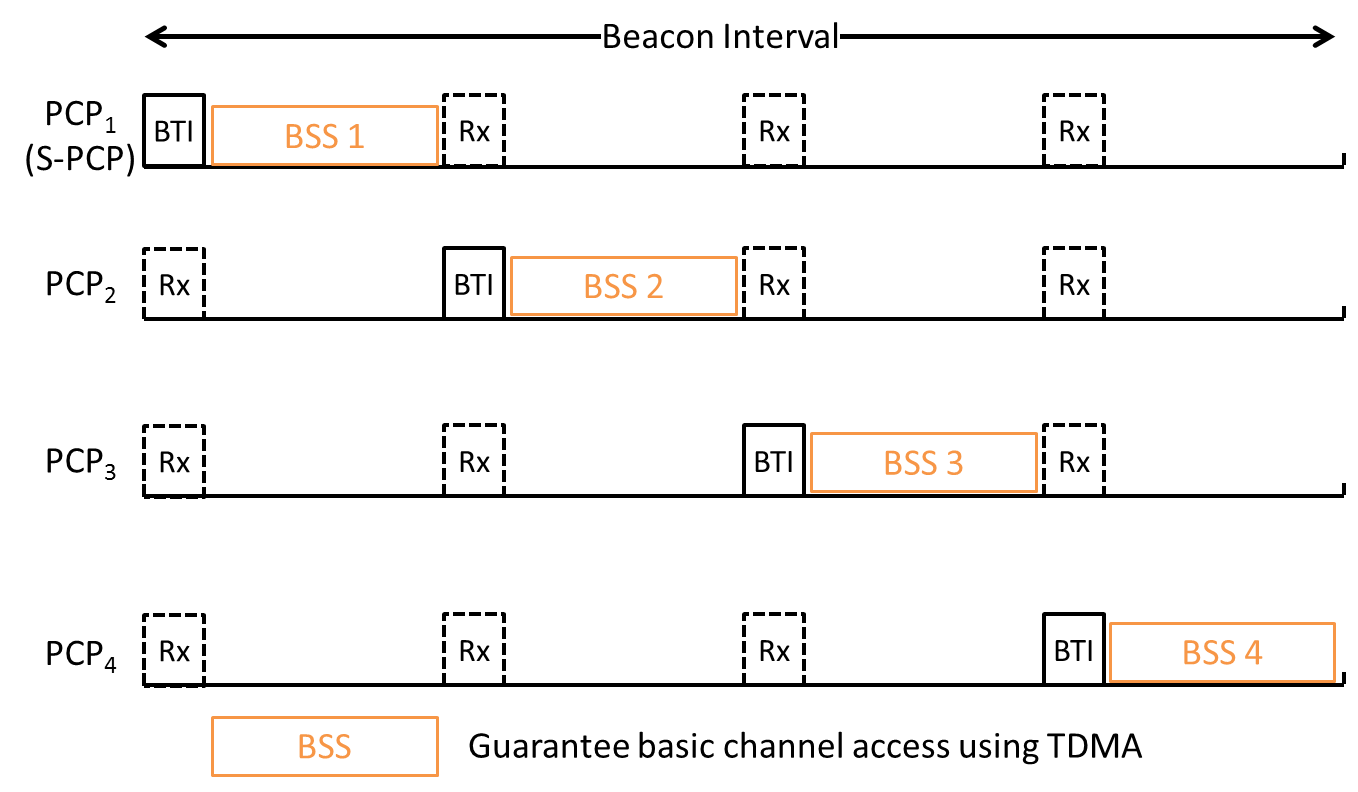
\includegraphics[width = 0.4\textwidth]{Clustering_tdma.pdf}
	\caption{Distributed clustering with TDMA scheduling among cluster members.}
	\label{fig:clustering:tdma}
\end{figure}

The directional antennas in mmWave allow concurrent transmissions and directional MAC protocols \cite{cocurrentbf}(more required here..) has been proposed to solve the deafness problem and achieve higher resource reuse. In wearable networks, different devices may have heterogeneous QoS requirements and the number of interferers can be large. To better guarantee the QoS requirements of different BSSs and different devices, we propose a hierarchical MAC for wearable networks with clustering.

In wearble networks, most transmissions within the PBSS are between the PCP and non-PCP devices. We denote primary transmissions as the transmissions between the PCP and the wearable devices with (highly) directional antennas and high QoS requirements, e.g., augmented reality devices. Secondary transmissions are between the PCP and the wearable devices with semi/omni-directional antennas with low QoS requirements like fitness trackers. 

\begin{figure}
	\centering
	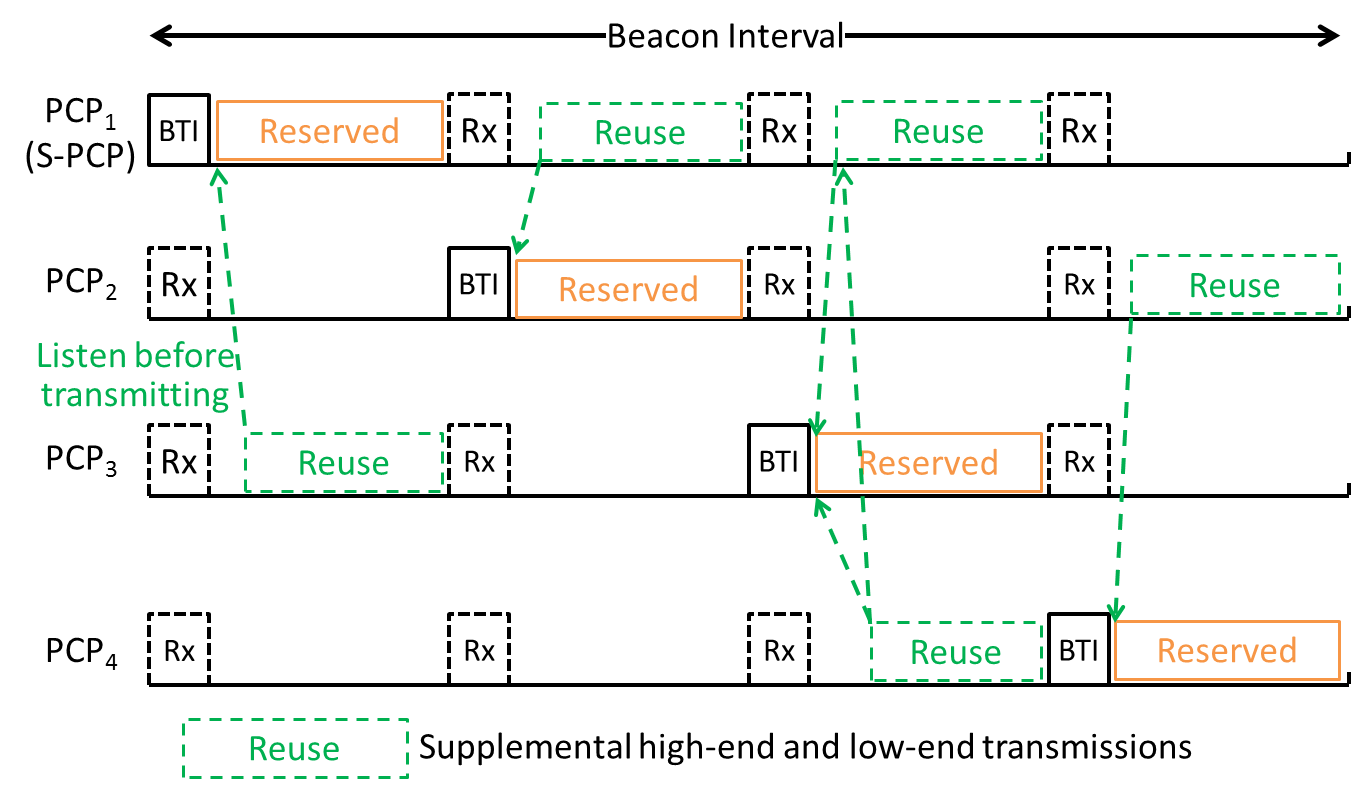
\includegraphics[width = 0.4\textwidth]{Clustering_reuse.pdf}
	\caption{Distributed clustering  with contention-based scheduling which achieves higher resource reuse.}
	\label{fig:clustering:reuse}
\end{figure}

To guarantee basic channel access and QoS of high-end transmissions, each PBSS is allocated with some reserved slots on which the PBSS is the primary PBSS and has higher transmission priority than other BSSs in the cluster, see Fig. \ref{fig:clustering:reuse}. The PBSS schedules its primary transmissions and (secondary transmissions if there is slots left) in its reserved slots. At the beginning of the its reserved slots, the PBSS sends directional RTS/CTS while other BSSs listen to the RTS/CTS of PBSS in the direction that otherwise the BSSs would use for transmission. After the primary user sends its RTS/CTS, other BSSs would try to reuse the channel according to their priorities either assigned by S-PCP or determined by sequence of the Beacon SPs. The PBSS with the highest priority will send the RTS/CTS if it does not interfere with the primary PBSS. The remaining BSSs listens to the RTS/CTS and try further reuse the channel according to their priorities. 

In our settings, the transmissions are within the BSSs and scheduled by the PCPs, thus there is no deafness problem. Also note that the transmissions of each PBSS is scheduled and broadcast in the beacon sent in the PBSS's Beacon SP, thus the BSSs know the transmissions scheduled in each slot and can use directional antenna to listen to the directional RTS/CTS. 


\section{Analysis of Clustering}\label{section:clusteranalysis}
In this section, we use an analytical model to evaluate the performance of clustering and channel selection for different scenarios based on our model for interference.

\subsection{System Model for cluster analysis}
We consider the performance of PBSSs in a typical cluster following the clustering principles we propose. Users are located on a 2-D plane following a HPPP with density $\lambda$. The cluster size is $K$ and there are $M$ channels. 
The power receiver $i$ receives from transmitter $j$ is given as follows, 
\begin{equation*}
P_r(j,i) = P_t(j)\cdot G_t(j,i) \cdot G_r(i,j) \cdot PL(i,j).
\end{equation*} 
where $P_t$ is the transmit power of $j$.

We consider both the LOS channel and reflection over the ceiling in our analysis and use the channels between PCPs to approximate the channels between PBSSs. If there is a LOS channel between two users, path loss is approximated by the path loss of LOS channel. If the LOS channel is blocked but there is a clear reflected channel over the ceiling, path loss is approximated by the reflected channel. Path loss is 0 if both paths are blocked.
The PL of a channel with length $d$ is as follows, 
\begin{equation*}
PL(d) = 
\begin{cases}
PL_{\LOS}(d), & w.p. ~ \mathrm{P_{LOS}}(d)\\
PL_{\mathrm{reflection}}(d), & w.p. ~ \mathrm{P_{reflection}}(d) - \mathrm{P_{LOS}}(d) \\
0, & w.p. ~ 1-\mathrm{P_{reflection}}(d)
\end{cases},
\end{equation*}
where $PL_{\LOS}(d)$ and $PL_{\mathrm{reflection}}(d)$ are the path loss of LOS channel and reflected channel respectively, $\mathrm{P_{LOS}}(d)$ is the probability of having a LOS channel, $\mathrm{P_{reflection}}(d)$ is the probability of having a clear reflected channel. The detailed channel model follows our analysis in Section \ref{section:channel}. 

The antenna gain of directional antennas is modeled using a sector antenna model.%, see Fig. \ref{fig:clusteringanalysis:antenna}. 
The width of the main lobe is $\theta_t$ and $\theta_r$, for transmit antenna and receive antenna respectively. The antenna gain in the main lobe is $M_t$ and $M_r$ and the gain in the main lobe is $m_t$ and $m_r$.

The transmitter and receiver of a link within a PBSS point their antennas to each other while other transmitters points their beams to a random direction uniformly distributed in $[0, 2\pi]$, thus the antenna gain is given as follows,
\begin{equation*}
G_t(j,i) = 
\begin{cases}
M_t(j), & w.p. ~ \theta_t(j)/2\pi \\
m_t(j), & w.p. ~ 1-\theta_t(j)/2\pi
\end{cases},
\end{equation*}
\begin{equation*}
G_r(i,j) = 
\begin{cases}
M_r(i), & w.p. ~ \theta_r(i)/2\pi \\
m_r(i), & w.p. ~ 1-\theta_r(i)/2\pi
\end{cases},
\end{equation*}
The transmission is successful if there is no other transmitters such that the power received at the receiver exceeds some threshold, i.e., $P_r(i,j)< P_{\mathrm{threshold}}, ~ \forall j$. $P_{\mathrm{threshold}}$ depends on the type of traffic. 

In each PBSS, there are three types of transmissions with different directionality and transmit power as follows,
\begin{itemize}
	\item Beacon: omni-directional, high power
	\item Primary: directional, high power
	\item Secondary: omni-directional, Low power
\end{itemize}

%For each type of traffic, the directions of transmissions, i.e., from PCP to other devices or from non-PCP devices to PCP, affects transmit power $P_t$, the gain of antennas $G$ and beam width $\theta$.

%Note that the transmit power, beam width and beam gain are related to the transmission type of $j$, which is influenced by the scheduling, clustering, as well as the traffic patterns of users.

After describing the model for channel and devices, we now introduce the model for MAC. 
The cluster head of the typical cluster is located at the origin $0$, with $K-1$ cluster members randomly distributed in the disc centered at $0$, see Fig. \ref{fig:clusteranalysis:model}. The radius of the disc, $R_{\mathrm{cluster}}$, satisfies that 
\begin{align*}
\lambda\pi (R_{\mathrm{cluster}}^2 - r_{\min}^2) = K - 1,\\
R_{\mathrm{cluster}} = \sqrt{\frac{K - 1}{\lambda\pi}+r_{\min}^2}.
\end{align*}
Channel selection makes neighboring clusters work on different channels and forms an inter-cluster interference protection region around the cluster with radius, 
\begin{equation*}
R_{\mathrm{protect}} = \sqrt{\frac{M\cdot K - 1}{\lambda \pi} + r_{\min}^2}.
\end{equation*}
All other users working on the same channel, i.e., the inter-cluster interferers, are distributed outside of the protection region following a HPPP with density $\frac{\lambda}{M}$ and work independently.

\begin{figure}
	\centering
	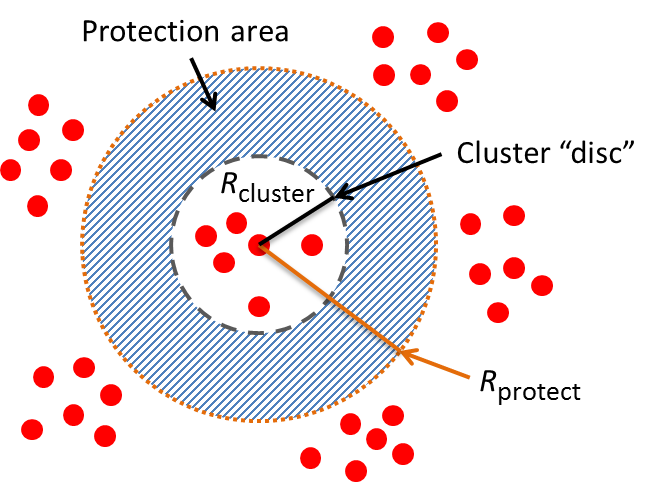
\includegraphics[width = 0.4\textwidth]{Clustering_model.pdf}
	\caption{Model of a typical cluster using clustering and channel selection. Red circles represent users working on the same channel.}
	\label{fig:clusteranalysis:model}
\end{figure}

We define that a transmission of a PBSS is interfered by a transmission from another PBSS if the signal received at the receiver of the transmission exceeds a threshold, $P_{\mathrm{threshold}}$. 
Two transmissions of two PBSSs interfere with each other if either transmission is interfered by the other transmission. 
A transmission fails if it is interfered by another transmission. Two transmissions can not be scheduled in the same slot if they interfere with each other and belong to PBSSs of the same cluster.

Denote $T_{\mathrm{frame}}$ as the length of frame and $T_{\mathrm{beacon}}$ as the length of one Beacon SP. The cluster head reserves exact $K$ Beacon SPs thus $K\cdot T_{\mathrm{beacon}}$ is reserved for beacon transmission in each frame and $T_{\mathrm{data}} = T_{\mathrm{frame}} - K\cdot T_{\mathrm{beacon}}$ is used for data transmission. The proportion of data reserved for data transmission is given by
\begin{equation*}
p_{\mathrm{data}} = \frac{T_{\mathrm{data}}}{T_{\mathrm{frame}}}.
\end{equation*}
In each Beacon SP, the PCP of exactly one PBSS of the cluster will transmit its beacon and the other devices will receive the beacon using omni-directional mode. 

We assume that the PBSSs are full-buffer and try to schedule transmission in all slots. A PBSS schedules transmissions in its beacon period and will not change the scheduling until its next beacon period. PBSSs do not support concurrent transmission within a PBSS thus there is at most one transmission in a PBSS. Each user will schedule primary transmissions in a proportion of $\rho_{\mathrm{primary}}\in[0,1]$ of slots for data transmission and schedule secondary transmissions in the rest $\rho_{\mathrm{secondary}} =1 - \rho_{\mathrm{primary}}$ proportion of the slots. 

We consider two types of scheduling within the cluster, TDMA and hierarchical resource reuse (HRR). In TDMA scheduling, PBSSs share the slots equally within the cluster and the fraction of time that a PBSS can access the channel in a frame is given by, 
\begin{equation*}
p_{\mathrm{access}}^{\mathrm{TDMA}} = p_{\mathrm{data}}/K.
\end{equation*}
A PBSS will schedule primary transmissions in $\rho_{\mathrm{primary}}p_{\mathrm{data}}/K$ slots, and secondary transmissions in $(1-\rho_{\mathrm{primary}})p_{\mathrm{data}}/K$ of the slots. 

In HRR, each PBSS is allocated $1/K$ of the slots for data transmission in a frame where the PBSS has higher priority than other PBSSs in the cluster. The PBSS first schedules primary transmission in the reserved slots and schedules other transmissions by reusing the slots allocated to other PBSSs. If $\rho_{\mathrm{primary}}\leq 1/K$, the PBSS also schedules secondary transmissions in the allocated slots. 

In the allocated $1/K$ of the slots, the PBSS has the access to the channel. When trying to reuse other slots, the PBSS shall not interfere with the transmissions of the original user in the slots and share the channel with other PBSSs.
The probability that a PBSS can reuse the slots in approximated by
\begin{equation*}
\mathrm{P}_{\mathrm{clear}}\cdot \frac{1}{1+\E[N_{\mathrm{intra-cluster}}']},
\end{equation*}
where $\mathrm{P}_{\mathrm{clear}}$ is the probability that the PBSS does not interfere with the PBSS owning the slots, $\E[N_{\mathrm{intra-cluster}}']$ is the expected number of PBSSs in the cluster that also try to reuse the slots and interferes with the transmission.

\% Stop here on 11/30
%we assume there is an ideal resource sharing mechanism among the PBSSs in the cluster, i.e., independent set scheduling [ref required]. Let $N_{\mathrm{intra-cluster}}$ be the number of other PBSSs in the same cluster that interferes with the data transmission of PBSS at some slot for data transmission. $N_{\mathrm{intra-cluster}}$ is related to the type of transmission scheduled by the PBSS as well as the type of transmissions of other PBSSs. The probability that the transmission is scheduled can be approximated by, 
%\begin{equation*}
%p_{\mathrm{access}}^{\mathrm{IRR}} = p_{\mathrm{data}}/(1+\E[N_{\mathrm{intra-cluster}}]).
%\end{equation*} 
% proportion of different types of traffic \\
% $E[N_{intra-cluster}]$

A PBSS's transmission is successful if the transmission is not interfered by transmissions outside the cluster. Denote $N_{\mathrm{inter-cluster}}$ as the number of transmissions outside the cluster that interfere the transmission. Inter-cluster interferers are mutually independent and the spatial distribution follows HPPP thus $N_{\mathrm{inter-cluster}}$ follows poisson distribution. The probability of successful transmission is then approximated as follows, 
\begin{equation*}
p_{\mathrm{success}} = e^{-\E[N_{\mathrm{inter-cluster}}]}.
\end{equation*} 

$N_{\mathrm{intra-cluster}}$ is related to the transmission patterns of users, which depends on the distances to other PBSSs within the cluster. PBSSs located at different locations have different transmission patterns. We use the transmission pattern of a user $\sqrt{2}R_{\mathrm{cluster}}$ away from the cluster head as the typical transmission pattern for inter-cluster interferers to get the $\E[N_{\mathrm{inter-cluster}}]$.

Based on the above analysis, we can evaluate the throughput of a PBSS using the average successful transmission time (STT) of the user,
\begin{equation*}
STT = p_{\mathrm{data}}\times p_{\mathrm{access}} \times p_{\mathrm{success}}.
\end{equation*}

\subsection{Numerical Results and Discussion}
In this section, we compute the STT for different scenarios and characterize the optimal cluster size that maximizes the sum STT of users. 
The parameters used are listed in Table \ref{tab:clusteranalysis:parameter}.

\begin{table}
	\centering
	\caption{The parameters used for numerical analysis}
	\begin{tabular}{cc}
		\hline
		Parameter & Value \\
		\hline
		M & 4 \\
		$h_{\mathrm{ceiling}}$ & 2.8 m \\
		$\Gamma_{\mathrm{ceilin}}$ & 0.4654 \\
		$\lambda$ & 1 $\mathrm{user/m^2}$ \\
		$P_t^{\mathrm{high}}$ & 10 dBm \\
		$P_t^{\mathrm{low}}$ & 4 dBm \\
		$P_{\mathrm{threshold}}$ & -78 dBm \\
		$\rho_{\mathrm{primary}}$ & 0.5 \\
		$M_t$,$M_r$ ($\theta = 60\degree$) & 5 dB \\
		$m_t$,$m_r$ ($\theta = 60\degree$) & -5 dB \\
		$M_t$,$M_r$ ($\theta = 24\degree$) & 10 dB \\
		$m_t$,$m_r$ ($\theta = 24\degree$) & -10 dB \\		
		$T_{\mathrm{frame}}$ & 100 ms \\
		$T_{\mathrm{beacon}}$ & 2 ms \\
		\hline
	\end{tabular}
	\label{tab:clusteranalysis:parameter}	
\end{table}
% SINR not considered thus don't need noise figure ? 

In Fig. \ref{fig:clusteranalysis:basic} we show how $STT$ and $p_{\mathrm{success}}$ change with cluster size for the use located at the center of the cluster.  $p_{\mathrm{success}}$ increases with $K$ while $p_{\mathrm{data}}$ and $p_{\mathrm{access}}$ decreases. STT first increases with $K$, then saturates and decreases, indicating that large clusters may not provide good inter-cluster mitigation but increases the contention between users within the same cluster and signaling overhead. The STT of primary transmissions is maximized when cluster size is small while the STT of secondary transmissions is maximized at larger $K$, showing that secondary transmissions benefit more from interference mitigation of larger clusters.  

\begin{figure}[htp]
	\centering
	\subfloat[Successful transmission time (STT)]{\label{subfig:basic_stt} 									\includegraphics[width=0.4\textwidth]{Cluster_analysis_basic_stt.pdf} }
	
	\subfloat[Probability of successful transmission $p_{\mathrm{success}}$]{\label{subfig:basic_psuccess} \includegraphics[width=0.4\textwidth]{Cluster_analysis_basic_psuccess.pdf}}
	
	\caption[]{STT for data transmission \subref{subfig:basic_stt} and $p_{\mathrm{success}}$ \subref{subfig:basic_psuccess} for different cluster sizes. $\theta=60\degree$, $\rho_{\mathrm{primary}} = 0.5$. }
	\label{fig:clusteranalysis:basic}
\end{figure}

In Fig. \ref{fig:clusteranalysis:directionality} we compares STT when the antennas of primary transmissions have different directionality. Results show that when antennas are highly directional, the optimal cluster size is smaller. The results suggest that highly directional devices are less dependent on clustering to mitigate interference, thus users with highly directional devices may favor small clusters or not joining clusters. 
\begin{figure}
	\centering
	\includegraphics[width = 0.4\textwidth]{Cluster_analysis_directionality.pdf}
	\caption{STT for antennas with different directionality.}
	\label{fig:clusteranalysis:directionality}
\end{figure}

In Fig. \ref{fig:clusteranalysis:primary_ratio} we present the STT when users have different proportions of primary transmissions, $\rho_{\mathrm{primary}}$. Similar to our findings for Fig. \ref{fig:clusteranalysis:directionality}, directional transmissions requires smaller cluster size thus having more primary transmissions will decrease the optimal cluster size while in networks with more secondary transmissions, e.g., network with many active small wearable devices, larger cluster is required to reduce uncoordinated inter-cluster interference. 

\begin{figure}
	\centering
	\includegraphics[width = 0.4\textwidth]{Cluster_analysis_primary_ratio.pdf}
	\caption{STT for different tranffic patterns $\rho_{\mathrm{primary}}$.}
	\label{fig:clusteranalysis:primary_ratio}
\end{figure}

In Fig. \ref{fig:clusteranalysis:location} we compare the STT for users at different locations of the cluster.
The user located at the center and the edge do not differ much in STT but we can see that in large clusters, the STT of edge user is higher than that of center user. The reason is that when cluster size increases, $N_{\mathrm{intra-cluster}}$ increases faster for user at the center thus STT is smaller. However, edge users experience have more inter-cluster interferers thus in small clusters, the STT of edge users is smaller. This observation further supports our idea that setting the cluster size involves the trade-off between interference mitigation and resource reuse.

\begin{figure}
	\centering
	\includegraphics[width = 0.4\textwidth]{Cluster_analysis_location.pdf}
	\caption{STT for users at different locations: user located at the center of the cluster (Center) and user that is $R_{\mathrm{cluster}}$ from the center.}
	\label{fig:clusteranalysis:location}
\end{figure}


In Fig. \ref{fig:clustereanalysis:optimal_cluster_size} we show how the optimal cluster size that maximizes STT changes with user densities. When user density is high, the optimal cluster size does not change very much, indicating that optimal cluster size is pretty robust to user densities. However, as we have discussed, the directionality and proportion of different types of traffic influence the optimal cluster size. 

\begin{figure}
	\centering
	\includegraphics[width = 0.4\textwidth]{Cluster_analysis_optimal_cluster_size.pdf}
	\caption{Cluster size that maximizes STT for different user densities.}
	\label{fig:clustereanalysis:optimal_cluster_size}
\end{figure}

In Fig. \ref{fig:clusteranalysis:compare_mac} we compare the STT for different MAC protocols for different user densities. At each user density, the cluster size is chosen as the one that maximizes the total STT. For Aloha, users select channel randomly and the access probability is optimized to maximize total STT. Our first observation is that clustering and reuse provide moderate gain in STT, partly due to beacon overheads, but improves the probability of successful transmission. Our second observation is that the total STT first decreases with user density then starts to increase with density. Such a result is in line with our analysis of the interference environment that in very dense networks, close neighbors blocks the interference from distant interferers thus the interference in dense environment may not be the worst case. Our observation comes from the MAC perspective, and in fact sum interference will keep increasing with user density, although the increasing speed is smaller at high user densities. 

\begin{figure}
	\centering
	\includegraphics[width = 0.4\textwidth]{Cluster_analysis_compare_mac.pdf}
	\caption{Sum STT in different user densities for different MAC protocols, optimal Aloha, Cluster + TDMA and Cluster + IRR.}
	\label{fig:clusteranalysis:compare_mac}
\end{figure}

\%Conclusion for analysis of clusters?

\section{Conclusion}\label{section:conclusion}
Our analysis of strong interferers show that enabling mmWave wearable networks in high user densities does seem feasible from MAC design perspective. Blockage and directionality help limit the number of strong interferers to a few that are close by. PBSSs may coordinate with close neighbors through coarse grain coordination at reasonable overheads while treating interference from distant PBSSs as 
noise. However, the fast changing nature due to self-blockage and movements still pose challenges on tracking and coordinating of interferers. For relative stationary network, clustering with resource reuse works as a viable solution to coordinating the PBSSs. Finding the optimal cluster size requires trade-off between interference mitigation and resource reuse within cluster thus an ideal cluster protocol should adapt to different environment. When users are highly mobile, the channel changes very fast and it is hard to maintain the cluster thus the PBSSs may just work on its own instead of joining clusters. 

\appendix[Proof of generalised Steiner formula]
In this part we present the proof of generalized Steiner formula in \cite{stochasticapp}. In the proof we need the following two lemmas. 
\begin{lemma}\label{lemma:characterization}
	(Hadwiger's Characterization Theorem) Every non-negative, motion-invariant, monotone, C-additive convex body function $h$ can be written in the form, 
	\begin{equation}\label{characterization}
	h(K) = \sum\limits_{k=0}^{d}a_kV_k(K),
	\end{equation}
	where $a_k$ are non-negative constants depending on $h$.
\end{lemma}
\begin{lemma}\label{lemma:steiner}
	If the intrinsic volumes of $\Xi$, $V_k(\Xi)$, have finite first moments,
	\begin{equation*}
	\overbar{V}_k(\Xi) = \E[V_k(\Xi)]<\infty,
	\end{equation*}
	for $k=0,1,\ldots, d$, then Steiner formula is satisfied for $\Xi$ almost surely. For $r\geq 0$, 
	\begin{equation}
	\E[\nu_d(\Xi \oplus b(0,r))] = \sum\limits_{k=0}^{d}b_{d-k}\overbar{V}_k(\Xi)r^{d-k}.
	\end{equation}
\end{lemma}

\begin{theorem}
	For convex and isotropic $\Xi$, $\Xi$ has a distribution invariant w.r.t. rotations about the origin $0$, the generalized Steiner formula holds for every compact convex set $K$. 
	\begin{equation}
	\E\big[\nu_d(\Xi\oplus K)\big] = \frac{1}{b_d}\sum\limits_{k=0}^{d}\frac{b_k b_{d-k}}{{d \choose k}}\overbar{V}_k(\Xi) V_{d-k}(K).
	\end{equation}
\end{theorem}
\begin{proof}
	$\Xi$ is convex and isotropic, thus $h(K)$ satisfies Lemma \ref{lemma:characterization}. Let $h(K) = \E[\nu_d(\Xi \oplus K)]$ then by (\ref{characterization}) we have, 
	\begin{equation}\label{characterization:steiner}
	\E[\nu_d(\Xi\oplus K)] = \sum\limits_{k=0}^{d}a_kV_k(K),
	\end{equation}
	where $a_k$ are constants related to $k$ and $\Xi$ and hold for all $K$. 
	
	Let $K=b(0, r)$, then 
	\begin{equation}\label{characterization:ball}
	\begin{aligned}
	\E[\nu_d(\Xi\oplus b(0,r))] &= \sum\limits_{k=0}^{d}a_kV_k(b(0,r))\\
	& = \sum\limits_{k=0}^{d} a_k{d \choose k}\frac{b_d}{b_{d-k}}r^k,
	\end{aligned}
	\end{equation}
	for all $r\geq 0$.
	
	By Lemma \ref{lemma:steiner}, 
	\begin{equation}\label{steiner:ball}
	\begin{aligned}
	\E[\nu_d(\Xi\oplus b(0,r))] &= \sum\limits_{k=0}^{d}b_{d-k}\overbar{V}_k(\Xi)r^{d-k}\\
	& = \sum\limits_{k=0}^{d}b_k\overbar{V}_{d-k}(\Xi)r^k,
	\end{aligned}
	\end{equation}
	for all $r\geq 0$.
	
	By (\ref{characterization:ball}) and (\ref{steiner:ball}) and the equality of polynomials, we have 
	\begin{equation*}
	a_k{d \choose k}\frac{b_d}{b_{d-k}} = b_k\overbar{V}_{d-k}(\Xi),
	\end{equation*}
	for $k = 0, 1,\ldots, d$. ${d\choose k} = {d\choose {d-k}}$ thus
	\begin{equation}\label{ak}
	a_k = \frac{1}{b_d}\frac{b_kb_{d-k}}{{d\choose {d-k}}}\overbar{V}_{d-k}(\Xi),
	\end{equation}
	for $k = 0, 1,\ldots, d$. Replace the $a_k$ in (\ref{characterization:steiner}) with (\ref{ak}) then we prove the theorem.
\end{proof}

\begin{thebibliography}{50}
\bibitem{wearable}
``Smart Wearable Devices: Fitness, Glasses, Watches, Multimedia, Clothing, Jewellery, Healthcare \& Enterprise 2014-2019,'' \emph{Juniper Research}, Aug. 2014.

\bibitem{80211ad}
\emph{``IEEE Standard for Information Technology — Telecommunications and Information Exchange between Systems — Local and Metropolitan Area Networks — Specific Requirements. Part 11: Wireless MAN Medium Access Control (MAC) and Physical Layer (PHY) Specifications Amendment 3: Enhancements for Very High Throughput in 60 GHz Band,''}, IEEE Standard 802.11ad, 2012.

\bibitem{802153c}
\emph{``IEEE Standard for Information Technology — Telecommunications and Information Exchange between Systems — Local and Metropolitan Area Networks — Specific Requirements. Part 15.3: Wireless Medium Access Control (MAC) and Physical Layer (PHY) Specifications for High Rate Wireless Personal Area Networks (WPANs) Amendment 2: Millimeter-Wave-Based Alternative Physical Layer Extension,''} IEEE Std 802.15.3c, 2009.

\bibitem{ECMA387}
\emph{``High Rate 60 GHz PHY, MAC and PALs,''} ECMA Standard 387, 2010.

%\bibitem{mmwave_propagation}
%S. Y. Geng, J. Kivinen, X. W. Zhao, and P. Vainikainen, ``Millimeter-wave propagation channel characterization for short-range wireless communications,'' \emph{IEEE Trans. Veh. Tachnol.}, vol. 58, no. 1, pp. 3-13, Jan. 2009.

\bibitem{humanshadowing}
C. Gustafson and F. Tufvesson, \emph{``Characterization of 60 GHz Shadowing by Human Bodies and Simple Phantoms, ''} Antennas and Propagation (EUCAP), 6th European Conference on, 2012.

\bibitem{urbanblockage}
T. Bai and R.W. Heath Jr., ``Coverage and rate analysis for millimeter wave cellular networks,'' in \emph{IEEE Trans. Wireless Comm.}, vol. 13, no. 9, Sep. 2014.

\bibitem{interferencefinitesized}
K. Venugopal, M.C. Valenti and R.W. Heath, \emph{``Interference in Finite-Sized Highly Dense Millimeter Wave Networks,''} Information Theory and Applications Workshop, Feb. 2015.

\bibitem{enclosedmmwave}
G. George and A. Lozano, ``Performance of enclosed mmWave wearable networks,'' in IEEE Int'l Workshop on Compuational Advances in Multi-Sensor Adaptive Processing (CAMSAP 15), Dec. 2015. (Revision required)

\bibitem{humanactivity}
S. Collonge, G. Zaharia and G.E. Zein, ``Influence of human activity on wide-band characteristics of the 60 GHz indoor radio channel,'' \emph{IEEE Trans. Wirel. Commun.}, vol. 3,  no. 6, pp. 2369-2406, 2004.

\bibitem{timevaryingpathshadowing}
I. Kashiwagi, T. Taga and T. Imai, ``Time-varying path-shadowing model for indoor populated environments,'' \emph{IEEE Trans. Veh. Technol.}, vol. 59, no. 1, Jan. 2010.

\bibitem{blockagein60ghz}
S. Singh, F. Ziliotto, U. Madhow, E. M. Belding and M. Rodwell, ``Blockage and Directivity in 60 GHz Wireless Personal Area Networks: From Cross-Layer Model to Multihop MAC Design,'' \emph{IEEE J. Sel. Areas Commun.}, vol. 27, no. 8, Oct. 2009.


\bibitem{virtualtimeslot}
C. Sum, Z. Lan, R. Funada, J. Wang, T. Baykas, M. A. Rahman, and H. Harada, ``Virtual time-slot allocation scheme for throughput enhancement in a millimeter-wave multi-Gbps WPAN system,'' \emph{IEEE J. Sel. Areas Commun.}, vol. 27, no. 8, Oct. 2009.

\bibitem{rex}
L. X. Cai, L. Cai, X. Shen, and J. Mark, ``REX: a randomized exclusive region based scheduling scheme for mmWave WPANs with directional antenna,'' \emph{IEEE Trans Wireless Commun.}, vol. 9, no. 1, pp. 113-121, Jan. 2010. 

\bibitem{fdmac}
I. K. Son, S. Mao, M. X. Gong, and Y. Li, ``On frame-based scheduling for directional mmWave WPANs,'' in \emph{Proc. IEEE INFOCOM}, Orlando, FL, 2012, pp. 2149-2157.

\bibitem{dtdmac}
E. Shihab, L. Cai, and J. Pan, ``A distributed asynchronous directional-to-directional MAC protocol for wireless ad hoc networks,'' \emph{IEEE Tans. Veh. Tech.}, vol. 58, no. 9, pp. 5124-5134, Nov. 2009. 

\bibitem{mdmac}
S. Singh, R. Mudumbai, and U. Madhow, ``Distributed coordination with deaf neighbors: efficient medium access for 60 GHz mesh networks,'' in \emph{Proc. IEEE INFOCOM}, San Diego, CA, 2010, pp. 1-9.

%\bibitem{mmwaveadhoc}
%A. Thornburg, T. Bai and R.W. Heath Jr., ``Interference statistics in a random mmWave ad hoc network,'' in IEEE Int'l Conference on Acoustics, Speech and Signal Processing (ICASSP), Apr. 2015.

\bibitem{reflection}
K. Sato \emph{et al.}, ``Measurements of Reflection and Transmission Characteristics of Interior Structure of Office Building in the 60-GHz band,'' \emph{IEEE Trans. Antennas Propag.}, vol. 45, no. 12, pp. 1783-1792, Dec. 1997.

\bibitem{stochasticgeometry}
F. Baccelli and B. Blaszczyszyn, ``Stochastic geometry and wireless networks, volume \Rom{1} - theory,'' \emph{Foundations and Trends in Networking}, vol. 3, no. 3-4, pp. 249-449, 2009.

\bibitem{poisson}
J. F. C. Kingman, ``Poisson Processes,'' New York: The Clarendon Press Oxford Univ. Press, 1993.

\bibitem{stochasticapp}
S.N. Chiu, D. Stoyan, W.S. Kendall and J. Mecke, \emph{Stochastic Geometry and its Applications} (3rd ed). Hoboken: Wiley, 2013. 

\bibitem{busyperiod_heavytraffic}
P. Hall, ``Heavy Traffic Approximations for Busy Period in an M/G/$\infty$ Queue,'' \emph{Stochastic Processes and their Applications}, vol. 19, no. 2, pp. 259-269, 1985.

\bibitem{busyperiod_exponential}
M. A. M. Ferreira and M. Andrade, ``The M/G/$\infty$ Queue Busy Period Distribution Exponentiality,'' \emph{Applimat - Journal of Applied Mathematics}, vol. 4, no. 3, pp. 249-260, 2011.


\bibitem{matern}
B. Mat\'ern, Spatial Variation second ed. vol.36 of Lecture Notes in Statistics. (Revision required)

%\bibitem{backoff}
%H. Lee, H. Kwon, A. Motskin and  L. Guibas, \emph{``Interference-aware MAC Protocol for Wireless Networks by a Game-Theoretic Approach,''}, in \emph{INFOCOM}, Rio de Janeiro, 2009, pp. 1854-1862.

%\bibitem{apcluster}
%B.J. Frey and D. Dueck, \emph{``Clustering by Passing Messages Between Data Points,''} Science 315 (2007) 972-976.

%\bibitem{apvanet}
%B. Hassanabadi, C. Shea, L. Zhang and S. Valaee, \emph{``Clustering in Vehicular Ad Hoc Networks using Affinity Propagation,''} Ad Hoc Networks 13 (2014) 535-548.

%\bibitem{apd2d}
%D.J. Son, C.H. Yu and D.I Kim, \emph{``Resource Allocation based on Clustering for D2D Communications in Underlaying Cellular Networks,''} in \emph{Information and Communication Technology Convergence}, Busan, 2014, pp. 232-237.

\bibitem{onlinkscheduling}
Z. He, S. Mao and T.S. Rappaport, \emph{``On Link Scheduling Under Blockage and Interference in 60-GHz Ad Hoc Networks,''} edition required...

\bibitem{intersharing}
W. Feng, Y. Li, D. Jin and L. Zeng, \emph{``Inter-Network Spatial Sharing with Interference Mitigation Based on IEEE 802.11ad WLAN System,''} Globecom 2014 workshop - telecommunications standards - from research to standards

\bibitem{cocurrentbf}
J. Qiao, X. Shen, J.W. Mark and Y. He, \emph{``MAC-layer Concurrent Beamforming Protocol for Indoor Millimeter Wave Networks''}, in \emph{IEEE Trans. Veh. Tachnol.}, vol , no. ,   2014. 

\end{thebibliography}

\end{document}
